%
% chapter.tex -- Kapitel über Eigenwerte und Eigenvektoren
%
% (c) 2021 Prof Dr Andreas Müller, OST Ostschweizer Fachhochschule
%
\chapter{Eigenwerte und Eigenvektoren
\label{buch:chapter:eigenwerte-und-eigenvektoren}}
\lhead{Eigenwerte und Eigenvektoren}
\rhead{}
Die algebraischen Eigenschaften einer Matrix $A$ sind eng mit der
Frage nach linearen Beziehungen unter den Potenzen von $A^k$ verbunden.
Im Allgemeinen ist die Berechnung dieser Potenzen eher unübersichtlich,
es sei denn, die Matrix hat eine spezielle Form.
Die Potenzen einer Diagonalmatrix erhält man, indem man die Diagonalelemente
potenziert.
Auch für Dreiecksmatrizen ist mindestens die Berechnung der Diagonalelemente
von $A^k$ einfach.
Die Theorie der Eigenwerte und Eigenvektoren ermöglicht, Matrizen in
eine solche besonders einfache Form zu bringen.

In Abschnitt~\ref{buch:section:grundlagen} werden die grundlegenden
Definitionen der Eigenwerttheorie in Erinnerung gerufen.
Damit kann dann in Abschnitt~\ref{buch:section:normalformen}
gezeigt werden, wie Matrizen in besonders einfache Form gebracht
werden können.
Die Eigenwerte bestimmen auch die Eigenschaften von numerischen
Algorithmen, wie in den Abschnitten~\ref{buch:section:spektralradius}
und \ref{buch:section:numerisch} dargestellt wird.
Für viele Funktionen kann man auch den Wert $f(A)$ berechnen, unter
geeigneten Voraussetzungen an den Spektralradius.
Dies wird in Abschnitt~\ref{buch:section:spektraltheorie} beschrieben.


%
% grundlagen.tex -- Grundlagen
%
% (c) 2021 Prof Dr Andreas Müller, OST Ostschweizer Fachhochschule
%
\section{Grundlagen
\label{buch:section:grundlagen}}
\rhead{Grundlagen}
Die Potenzen $A^k$ sind besonders einfach zu berechnen, wenn die Matrix
Diagonalform hat, wenn also $A=\operatorname{diag}(\lambda_1,\dots,\lambda_n)$
ist.
In diesem Fall ist $Ae_k=\lambda_k e_k$ für jeden Standardbasisvektor $e_k$.
Statt sich auf Diagonalmatrizen zu beschränken könnten man also auch
Vektoren $v$ suchen, für die gilt $Av=\lambda v$, die also von $A$ nur
gestreckt werden.
Gelingt es, eine Basis aus solchen sogenanten {\em Eigenvektoren} zu finden,
dann kann man die Matrix $A$ durch Basiswechsel in diese Form bringen.

\begin{figure}
\centering
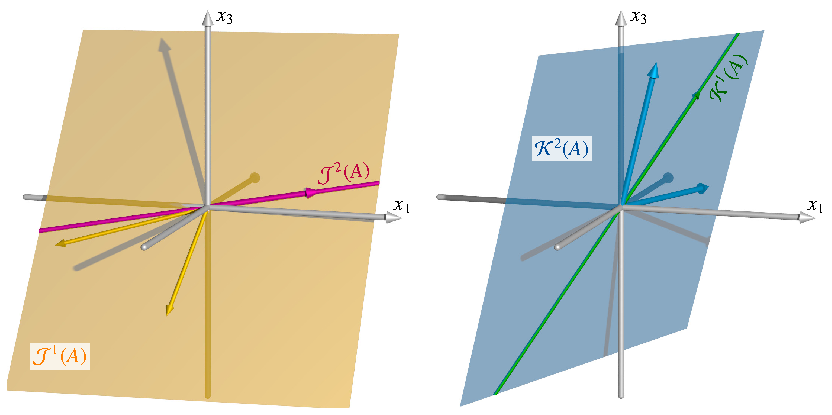
\includegraphics[width=\textwidth]{chapters/40-eigenwerte/images/kernbild.pdf}
\caption{Iterierte Kerne und Bilder einer $3\times 3$-Matrix mit Rang~2.
Die abnehmend geschachtelten iterierten Bilder
$\mathcal{J}^1(A) \subset \mathcal{J}^2(A)$
sind links dargestellt, die zunehmen geschachtelten iterierten Kerne
$\mathcal{K}^1(A) \subset \mathcal{K}^2(A)$ rechts.
\label{buch:eigenwerte:img:kernbild}}
\end{figure}

\begin{figure}
\centering
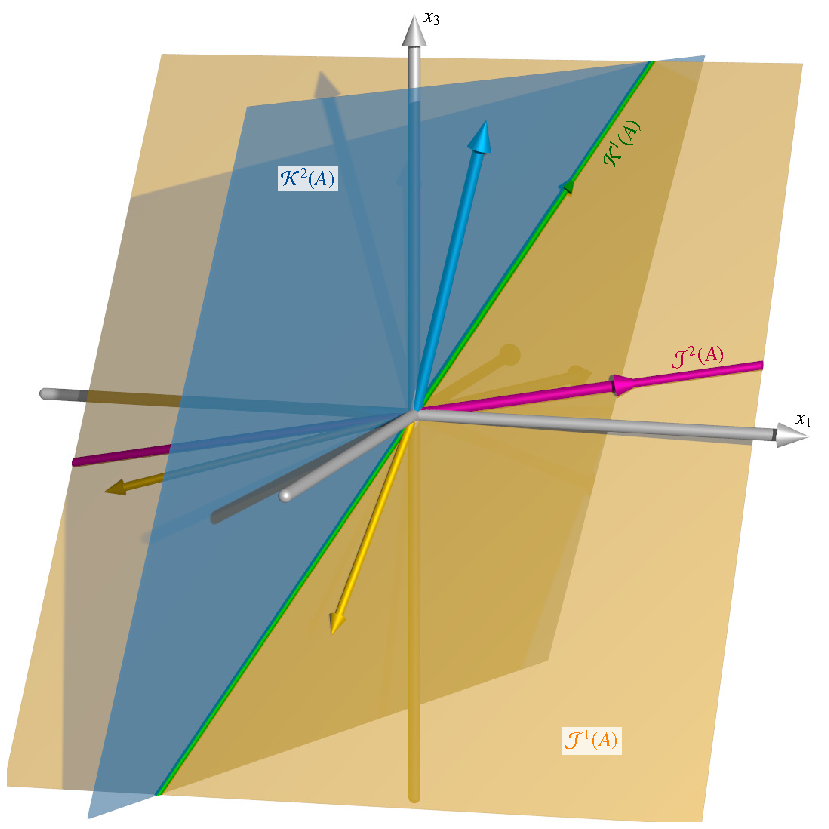
\includegraphics[width=\textwidth]{chapters/40-eigenwerte/images/kombiniert.pdf}
\caption{Iterierte Kerne und Bilder einer $3\times 3$-Matrix mit Rang~2.
Da $\dim\mathcal{J}^2(A)=1$ und $\dim\mathcal{J}^1(A)=2$ ist, muss es
einen Vektor in $\mathcal{J}^1(A)$ geben, der von $A$ auf $0$ abgebildet
wird, der also auch im Kern $\mathcal{K}^1(A)$ liegt.
Daher ist $\mathcal{K}^1(A)$ die Schnittgerade von $\mathcal{J}^1(A)$ und
$\mathcal{K}^2(A)$.
Man kann auch gut erkennen, dass
$\mathbb{R}^3
=
\mathcal{K}^1(A)\oplus \mathcal{J}^1(A)
=
\mathcal{K}^2(A) \oplus \mathcal{J}^2(A)$
ist.
\label{buch:eigenwerte:img:kombiniert}}
\end{figure}

%
% Kern und Bild von Matrixpotenzen
%
\subsection{Kern und Bild von Matrixpotenzen
\label{buch:subsection:kern-und-bild}}
In diesem Abschnitt ist $A\in M_n(\Bbbk)$, $A$ beschreibt eine lineare
Abbildung $f\colon\Bbbk^n\to \Bbbk^n$.
In diesem Abschnitt sollen Kern und Bild der Potenzen $A^k$ untersucht
werden.
\begin{definition}
Wir bezeichnen Kern und Bild der iterierten Abbildung $A^k$ mit
\[
\mathcal{K}^k(A)
=
\ker A^k
\qquad\text{und}\qquad
\mathcal{J}^k(A)
=
\operatorname{im} A^k.
\]
\end{definition}

Durch Iteration wird das Bild immer kleiner.
Wegen
\[
\mathcal{J}^k (A)
=
\operatorname{im} A^k
=
\operatorname{im} A^{k-1} A
=
\{ A^{k-1} Av\;|\; v \in \Bbbk^n\}
\subset
\{ A^{k-1} v\;|\; v \in \Bbbk^n\}
=
\mathcal{J}^{k-1}(A)
\]
folgt
\begin{equation}
\Bbbk^n
=
\operatorname{im}E
=
\operatorname{im}A^0
=
\mathcal{J}^0(A)
\supset
\mathcal{J}^1(A)
=
\operatorname{im}A
\supset
\mathcal{J}^2(A)
\supset\dots\supset
\mathcal{J}^k(A)
\supset
\mathcal{J}^{k+1}(A)
\supset \dots \supset
\{0\}.
\label{buch:eigenwerte:eqn:Jkchain}
\end{equation}
Für die Kerne gilt etwas Ähnliches.
Ein Vektor $x\in \mathcal{K}^k(A)$ erfüllt $A^kx=0$.
Dann erfüllt er aber erst recht auch
\[
A^{k+1}x=A\underbrace{A^kx}_{\displaystyle=0}=0,
\]
also ist $x\in\mathcal{K}^k(A)$.
Es folgt
\begin{equation}
\{0\}
=
\mathcal{K}^0(A) = \ker A^0 = \ker E
\subset
\mathcal{K}^1(A) = \ker A
\subset
\dots
\subset
\mathcal{K}^k(A)
\subset
\mathcal{K}^{k+1}(A)
\subset
\dots
\subset
\Bbbk^n.
\label{buch:eigenwerte:eqn:Kkchain}
\end{equation}
Neben diesen offensichtlichen Resultaten kann man aber noch mehr
sagen.
Es ist klar, dass in beiden Ketten
\label{buch:eigenwerte:eqn:Jkchain}
und
\label{buch:eigenwerte:eqn:Kkchain}
nur in höchstens $n$ Schritten eine wirkliche Änderung stattfinden 
kann.
Man kann aber sogar genau sagen, wo Änderungen stattfinden:

\begin{satz}
\label{buch:eigenwerte:satz:ketten}
Ist $A\in M_n(\Bbbk)$ eine $n\times n$-Matrix, dann gibt es eine Zahl $k$
so, dass
\[
\begin{array}{rcccccccccccl}
0=\mathcal{K}^0(A)
&\subsetneq& \mathcal{K}^1(A) &\subsetneq& \mathcal{K}^2(A)
&\subsetneq&\dots&\subsetneq&
\mathcal{K}^k(A) &=& \mathcal{K}^{k+1}(A) &=& \dots
\\
\Bbbk^n= \mathcal{J}^0(A)
&\supsetneq& \mathcal{J}^1(A) &\supsetneq& \mathcal{J}^2(A)
&\supsetneq&\dots&\supsetneq&
\mathcal{J}^k(A) &=& \mathcal{J}^{k+1}(A) &=& \dots
\end{array}
\]
ist.
\end{satz}

\begin{proof}[Beweis]
Es sind zwei Aussagen zu beweisen.
Erstens müssen wir zeigen, dass die Dimension von $\mathcal{K}^i(A)$ 
nicht mehr grösser werden kann, wenn sie zweimal hintereinander gleich war.
Nehmen wir daher an, dass $\mathcal{K}^i(A) = \mathcal{K}^{i+1}(A)$.
Wir müssen $\mathcal{K}^{i+2}(A)$ bestimmen.
$\mathcal{K}^{i+2}(A)$ besteht aus allen Vektoren $x\in\Bbbk^n$ derart,
dass $Ax\in \mathcal{K}^{i+1}(A)=\mathcal{K}^i(A)$ ist.
Daraus ergibt sich, dass $AA^ix=0$, also ist $x\in\mathcal{K}^{i+1}(A)$.
Wir erhalten also
$\mathcal{K}^{i+2}(A)\subset\mathcal{K}^{i+1}\subset\mathcal{K}^{i+2}(A)$,
dies ist nur möglich, wenn beide gleich sind.

Analog kann man für die Bilder vorgehen.
Wir nehmen an, dass $\mathcal{J}^i(A) = \mathcal{J}^{i+1}(A)$ und
bestimmten $\mathcal{J}^{i+2}(A)$.
$\mathcal{J}^{i+2}(A)$ besteht aus all jenen Vektoren, die als
$Ax$ mit $x\in\mathcal{J}^{i+1}(A)=\mathcal{J}^i(A)$ erhalten
werden können.
Es gibt also insbesondere ein $y\in\Bbbk^i$ mit $x=A^iy$.
Dann ist $Ax=A^{i+1}y\in\mathcal{J}^{i+1}(A)$.
Insbesondere besteht $\mathcal{J}^{i+2}(A)$ genau aus den Vektoren
von $\mathcal{J}^{i+1}(A)$.

Zweitens müssen wir zeigen, dass die beiden Ketten bei der gleichen
Potenz von $A$ konstant werden.
Dies folgt jedoch daraus, dass $\dim\mathcal{J}^i(A) = \operatorname{Rang} A^i
= n - \dim\ker A^i = n -\dim\mathcal{K}^i(A)$.
Der Raum $\mathcal{J}^k(A)$ hört also beim gleichen $i$ auf, kleiner
zu werden, bei dem auch $\mathcal{K}^i(A)$ aufhört, grösser zu werden.
\end{proof}

\begin{satz}
Die Zahl $k$ in Satz~\ref{buch:eigenwerte:satz:ketten}
ist nicht grösser als $n$, also
\[
\mathcal{K}^n(A) = \mathcal{K}^l(A)
\qquad\text{und}\qquad
\mathcal{J}^n(A) = \mathcal{J}^l(A)
\]
für $l\ge n$.
\end{satz}

\begin{proof}[Beweis]
Nach Satz~\ref{buch:eigenwerte:satz:ketten} muss die
Dimension von $\mathcal{K}^i(A)$ in jedem Schritt um mindestens
$1$ zunehmen, das ist nur möglich, bis zur Dimension $n$.
Somit können sich $\mathcal{K}^i(A)$ und $\mathcal{J}^i(A)$ für $i>n$
nicht mehr ändern.
\end{proof}

\begin{figure}
\centering
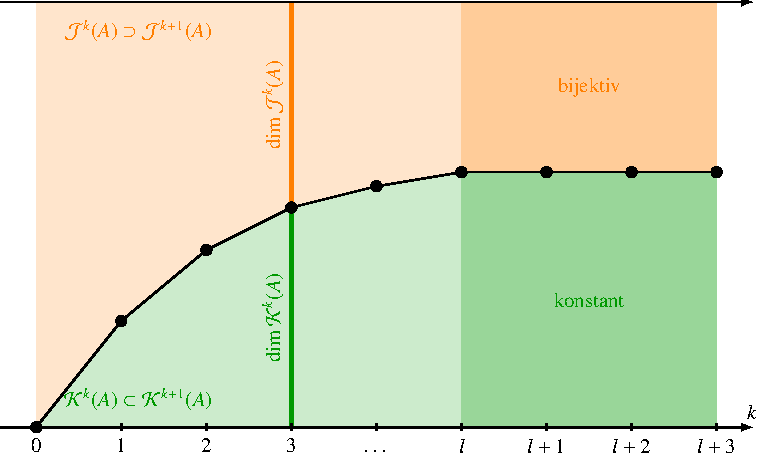
\includegraphics{chapters/40-eigenwerte/images/dimjk.pdf}
\caption{Entwicklung der Dimension von $\dim\mathcal{K}^k(A)$ (grün)
und $\dim\mathcal{J}^k(A)$ (orange) in Abhängigkeit vom Exponenten $k$.
Für $k\ge l$ ändern sich die Dimensionen nicht mehr, $A$ eingeschränkt
auf $\mathcal{J}^l(A)=\mathcal{J}(A)$ ist injektiv.
\label{buch:eigenwerte:fig:dimjk}}
\end{figure}

Abbildung~\ref{buch:eigenwerte:fig:dimjk} zeigt die Abhängigkeit der
Dimensionen $\dim\mathcal{K}^k(A)$ und $\dim\mathcal{J}^k(A)$ von $k$.
Die Dimension $\dim\mathcal{J}^k(A)$ nimmt ab bis zu $k=l$, danach ändert
sie sich nicht mehr und die Einschränkung von $A$ auf $\mathcal{J}^l(A)$ 
ist injektiv.
Die Dimension $\dim\mathcal{K}^k(A)$ nimmt zu bis zu $k=l$, danach
ändert sie sich nicht mehr.

\begin{definition}
\label{buch:eigenwerte:def:KundJ}
Die gemäss Satz~\ref{buch:eigenwerte:satz:ketten} identischen Unterräume
$\mathcal{K}^i(A)$ für $i\ge k$ und die identischen Unterräume
$\mathcal{J}^i(A)$ für $i\ge k$ werden mit
\[
\begin{aligned}
\mathcal{K} &= \mathcal{K}^i(A)&&\forall i\ge k \qquad\text{und}
\\
\mathcal{J} &= \mathcal{J}^i(A)&&\forall i\ge k
\end{aligned}
\]
bezeichnet.
\end{definition}


%
% Inveriante Unterräume
%
\subsection{Invariante Unterräume
\label{buch:subsection:invariante-unterraeume}}
Kern und Bild sind der erste Schritt zu einem besseren Verständnis 
einer linearen Abbildung oder ihrer Matrix.
Invariante Räume dienen dazu, eine lineare Abbildung in einfachere
Abbildungen zwischen ``kleineren'' Räumen zu zerlegen, wo sie leichter
analysiert werden können.

\begin{definition}
Sei $f\colon V\to V$ eine lineare Abbildung eines Vektorraums in sich
selbst.
Ein Unterraum $U\subset V$ heisst {\em invarianter Unterraum},
wenn
\[
f(U) = \{ f(x)\;|\; x\in U\} \subset U
\]
gilt.
\end{definition}

Der Kern $\ker A$  einer linearen Abbildung ist trivialerweise ein
invarianter Unterraum, da alle Vektoren in $\ker A$ auf $0\in\ker A$
abgebildet werden.
Ebenso ist natürlich $\operatorname{im}A$ ein invarianter Unterraum,
denn jeder Vektor wird in $\operatorname{im}A$ abgebildet, insbesondere
auch jeder Vektor in $\operatorname{im}A$.

\begin{satz}
\label{buch:eigenwerte:satz:KJinvariant}
Sei $f\colon V\to V$ eine lineare Abbildung mit Matrix $A$.
Jeder der Unterräume $\mathcal{J}^i(A)$ und $\mathcal{K}^i(A)$ 
ist ein invarianter Unterraum.
\end{satz}

\begin{proof}[Beweis]
Sei $x\in\mathcal{K}^i(A)$, es gilt also $A^ix=0$.
Wir müssen überprüfen, dass $Ax\in\mathcal{K}^i(A)$.
Wir berechnen daher $A^i\cdot Ax=A^{i+1}x=A\cdot A^ix = A\cdot 0=0$,
was zeigt, dass $Ax\in\mathcal{K}^i(A)$.

Sei jetzt $x\in\mathcal{J}^i(A)$, es gibt also ein $y\in V$ derart, dass
$A^iy=x$.
Wir müssen überprüfen, dass $Ax\in\mathcal{J}^i(A)$.
Dazu berechnen wir $Ax=AA^iy=A^iAy\in\mathcal{J}^i(A)$, $Ax$ ist also das
Bild von $Ay$ unter $A^i$.
\end{proof}

\begin{korollar}
Die Unterräume $\mathcal{K}(A)\subset V$ und $\mathcal{J}(A)\subset V$
sind invariante Unterräume.
\end{korollar}

Die beiden Unterräume $\mathcal{K}(A)$ und $\mathcal{J}(A)$ sind besonders
interessant, da wir aus der Einschränkung der Abbildung $f$ auf diese
Unterräume mehr über $f$ lernen können.

\begin{satz}
\label{buch:eigenwerte:satz:fJinj}
Die Einschränkung von $f$ auf $\mathcal{J}(A)$ ist injektiv.
\end{satz}

\begin{proof}[Beweis]
Die Einschränkung von $f$ auf $\mathcal{J}^k(A)$ ist
$\mathcal{J}^k(A) \to \mathcal{J}^{k+1}(A)$, nach Definition von
$\mathcal{J}^{k+1}(A)$ ist diese Abbildung surjektiv.
Da aber $\mathcal{J}^k(A)=\mathcal{J}^{k+1}(A)$ ist, ist
$f\colon \mathcal{J}^k(A)\to\mathcal{J}^k(A)$ surjektiv,
also ist $f$ auf $\mathcal{J}^k(A)$ auch injektiv.
\end{proof}

Die beiden Unterräume $\mathcal{J}(A)$ und $\mathcal{K}(A)$
sind Bild und Kern der iterierten Abbildung mit Matrix $A^k$.
Das bedeutet, dass $\dim\mathcal{J}(A)+\mathcal{K}(A)=n$.
Da $\mathcal{K}(A)=\ker A^k$ und andererseits $A$ injektiv ist auf
$\mathcal{J}(A)$, muss $\mathcal{J}(A)\cap\mathcal{K}(A)=0$.
Es folgt, dass $V=\mathcal{J}(A) + \mathcal{K}(A)$.

In $\mathcal{K}(A)$ und $\mathcal{J}(A)$ kann man unabhängig voneinander
jeweils eine Basis wählen.
Die Basen von $\mathcal{K}(A)$ und $\mathcal{J}(A)$ zusammen ergeben
eine Basis von $V$.
Die Matrix $A'$ in dieser Basis wird die Blockform
\[
A'
=
\left(
\begin{array}{ccc|ccc}
&&&&&\\
&A_{\mathcal{K}'}&&&&\\
&&&&&\\
\hline
&&&&&\\
&&&&A_{\mathcal{J}'}&\\
&&&&&\\
\end{array}
\right)
\]
haben, wobei die Matrix $A_\mathcal{J}'$ invertierbar ist.
Die Zerlegung in invariante Unterräume ergibt also eine natürlich
Aufteilung der Matrix $A$ in kleiner Matrizen mit zum Teil bekannten
Eigenschaften.

%
% Spezialfall, nilpotente Matrizen
%
\subsection{Nilpotente Matrizen
\label{buch:subsection:nilpotente-matrizen}}
Die Zerlegung von $V$ in die beiden invarianten Unterräume $\mathcal{J}(A)$
und $\mathcal{K}(A)$ reduziert die lineare Abbildung auf zwei Abbildungen
mit speziellen Eigenschaften.
Es wurde bereits in Satz~\label{buch:eigenwerte:satz:fJinj} gezeigt,
dass die Einschränkung auf $\mathcal{J}(A)$ injektiv ist.
Die Einschränkung auf $\mathcal{K}(A)$ bildet nach Definition alle
Vektoren nach $k$-facher Iteration auf $0$ ab, $A^k\mathcal{K}(A)=0$.
Solche Abbildungen haben eine speziellen Namen.

\begin{definition}
\label{buch:eigenwerte:def:nilpotent}
Eine Matrix $A$ heisst nilpotent, wenn es eine Zahl $k$ gibt, so dass
$A^k=0$.
\end{definition}

\begin{beispiel}
Obere (oder untere) Dreiecksmatrizen mit Nullen auf der Diagonalen
sind nilpotent.
Wir rechnen dies wie folgt nach.
Die Matrix $A$ mit Einträgen $a_{ij}$
\[
A=\begin{pmatrix}
  0   &a_{12}&a_{13}&\dots &a_{1,n-1}&a_{1n}   \\
  0   &  0   &a_{23}&\dots &a_{1,n-1}&a_{2n}   \\
  0   &  0   &  0   &\dots &a_{1,n-1}&a_{3n}   \\
\vdots&\vdots&\vdots&\ddots&\vdots   &\vdots   \\
  0   &  0   &  0   &\dots &  0      &a_{n-1,n}\\
  0   &  0   &  0   &\dots &  0      &  0
\end{pmatrix}
\]
erfüllt $a_{ij}=0$ für $i\ge j$.
Wir zeigen jetzt, dass sich bei der Multiplikation die nicht
verschwinden Elemente bei der Multiplikation noch rechts oben
verschieben.
Dazu multiplizieren wir zwei Matrizen $B$ und $C$ mit
$b_{ij}=0$ für $i+k>j$ und $c_{ij}=0$ für $i+l>j$.
In der folgenden graphischen Darstellung der Matrizen sind die
Bereiche, wo die Matrixelemente verschwinden, weiss.
\begin{center}
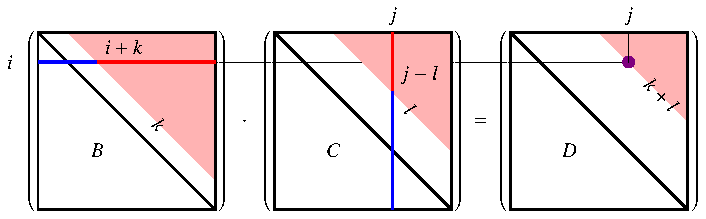
\includegraphics{chapters/40-eigenwerte/images/nilpotent.pdf}
\end{center}
Bei der Berechnung des Elementes $d_{ij}$ wird die Zeile $i$ von $B$
mit der Spalte $j$ von $C$ multipliziert.
Die blau eingefärbten Elemente in dieser Zeile und Spalte sind $0$.
Aus der Darstellung ist abzulesen, dass das Produkt verschwindet, 
die roten, von $0$ verschiedenen Elemente von den blauen Elementen
annihiliert werden.
Dies passiert immer, wenn $i+k>j-l$ ist, oder $i+(k+l)> j$.

Wir wenden diese Beobachtung jetzt auf die Potenzen $A^s$ an.
Für die Matrixelemente von $A^s$ schreiben wir $a^s_{ij}$.
Wir behaupten, dass die Matrixelemente $A^s$ die Bedingung
$a_{ij}^s=0$ für $i+s>j$ erfüllen.
Dies ist für $s=1$ nach Voraussetzung richtig, dies ist die
Induktionsvoraussetzung.
Nehmen wir jetzt an, dass $a_{ij}^s=0$ für $i+s>j$, dann folgt
aus obiger Rechnung, dass $a_{ij}^{s+1}=0$ für $i+s+1>j$, so
dass die Bedingung auch für $A^s$ gilt (Induktionsschritt).
Mit vollständiger Induktion folgt, dass $a_{ij}^s=0$ für $i+s>j$.
Insbesondere ist $A^n=0$, die Matrix $A$ ist nilpotent.
\end{beispiel}


Man kann die Konstruktion der Unterräume $\mathcal{K}^i(A)$ weiter
dazu verwenden, eine Basis zu finden, in der eine nilpotente Matrix
eine besonders einfach Form erhält.

\begin{satz}
\label{buch:eigenwerte:satz:nnilpotent}
Sei $A$ eine nilpotente $n\times n$-Matrix mit der Eigenschaft, dass
$A^{n-1}\ne 0$.
Dann gibt es eine Basis so, dass $A$ die Form
\begin{equation}
A'
=
\begin{pmatrix}
0&1& &      & & \\
 &0&1&      & & \\
 & &0&      & & \\
 & & &\ddots&1& \\
 & & &      &0&1\\
 & & &      & &0\\
\end{pmatrix}
\label{buch:eigenwerte:eqn:nnilpotent}
\end{equation}
bekommt.
\end{satz}

\begin{proof}[Beweis]
Da $A^{n-1}\ne 0$ ist, gibt es einen Vektor $b_n$ derart, dass $A^{n-1}b_n\ne0$.
Wir konstruieren die Vektoren
\[
b_n,\;
b_{n-1}=Ab_n,\;
b_{n-2}=Ab_{n-1},\;
\dots,\;
b_2=Ab_3,\;
b_1=Ab_2.
\]
Aus der Konstruktion folgt $b_1=A^{n-1}b_n\ne 0$, aber $Ab_1=A^nb_n=0$.
Aus der Konstruktion der iterierten Kerne $\mathcal{K}^i(A)$ folgt jetzt,
dass die Vektoren $b_1,\dots,b_n$ eine Basis bilden.
In dieser Basis hat die Matrix die Form~\ref{buch:eigenwerte:eqn:nnilpotent}.
\end{proof}

\begin{definition}
Wir bezeichnen mit $N_n$ eine Matrix der Form
\eqref{buch:eigenwerte:eqn:nnilpotent}.
\end{definition}

Mit etwas mehr Sorgfalt kann man auch die Bedingung, dass $A^{n-1}\ne 0$
sein muss, im Satz~\ref{buch:eigenwerte:satz:nnilpotent} loswerden.

\begin{satz}
\label{buch:eigenwerte:satz:allgnilpotent}
Sei $A$ ein nilpotente Matrix, dann gibt es eine Basis, in der die Matrix
aus lauter Nullen besteht ausser in den Einträgen unmittelbar oberhalb der 
Hauptdiagonalen, wo die Einträge $0$ oder $1$ sind.
Insbesondere zerfällt eine solche Matrix in Blöcke der Form $N_{k_i}$,
$i=1,\dots,l$,
wobei $k_1+\dots+k_l=n$ sein muss:
\begin{equation}
\def\temp#1{\multicolumn{1}{|c}{\raisebox{0pt}[17pt][12pt]{\phantom{x}$#1\mathstrut$}\phantom{x}}}
A'
=\left(
\begin{array}{cccc}
\cline{1-1}
\temp{N_{k_1}} &\multicolumn{1}{|c}{}&        &           \\
\cline{1-2}
          &\temp{N_{k_2}}&\multicolumn{1}{|c}{}&           \\
\cline{2-3}
          &           &\temp{\ddots}&\multicolumn{1}{|c}{}\\
\cline{3-4}
          &           &        &\multicolumn{1}{|c|}{\raisebox{0pt}[17pt][12pt]{\phantom{x}$N_{k_l}$}\phantom{x}}\\
\cline{4-4}
\end{array}
\right)
\label{buch:eigenwerte:eqn:allgnilpotent}
\end{equation}
\end{satz}

Die Einschränkung von $f$ auf den invarianten Unterraum $\mathcal{K}(A)$
ist nilpotent.
Die Zerlegung $V=\mathcal{J}(A)\oplus \mathcal{K}(A)$ führt also zu einer
Zerlegung der Abbildung $f$ in eine invertierbare Abbildung
$\mathcal{J}(A)\to\mathcal{J}(A)$ und eine
nilpotente Abbildung $\mathcal{K}(A)\to\mathcal{K}(A)$.
Nach Satz~\ref{buch:eigenwerte:satz:allgnilpotent} kann man in
$\mathcal{K}(A)$ eine Basis so wählen, dass die Matrix die Blockform
\eqref{buch:eigenwerte:eqn:allgnilpotent} erhält.



\begin{figure}
\centering
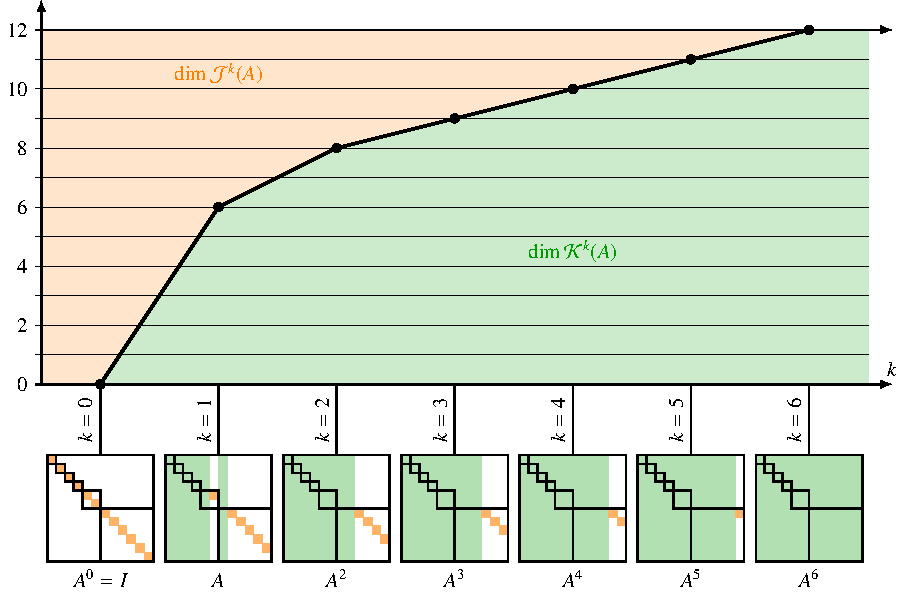
\includegraphics[width=\textwidth]{chapters/40-eigenwerte/images/jknilp.pdf}
\caption{Entwicklung der Dimensionen von Kern und Bild von $A^k$ in
Abhängigkeit von $k$
\label{buch:eigenwte:fig:jknilp}}
\end{figure}

\begin{beispiel}
In der Abbildung~\ref{buch:eigenwte:fig:jknilp} sind die Dimensionen
von Kern und Bild der Matrix
\[
\setcounter{MaxMatrixCols}{12}
A=\begin{pmatrix}
0& & & & & & & & & & & \\
 &0& & & & & & & & & & \\
 & &0& & & & & & & & & \\
 & & &0& & & & & & & & \\
 & & & &0&1& & & & & & \\
 & & & & &0& & & & & & \\
 & & & & & &0&1& & & & \\
 & & & & & & &0&1& & & \\
 & & & & & & & &0&1& & \\
 & & & & & & & & &0&1& \\
 & & & & & & & & & &0&
\end{pmatrix}
\]
dargestellt.
Die Matrix $A^k$ ist in den kleinen Quadraten am unteren Rand der Matrix
symbolisch dargestellt.
Grüne Spalten bestehen aus lauter Nullen, die zugehörigen
Standardbasisvektoren werden von diesem $A^k$ auf $0$ abgebildet.
Die orangen Felder enthalten Einsen, die entsprechenden Standardbasisvektoren
bilden daher eine Basis des Bildes von $A^k$.
\end{beispiel}

%
% Basis für die Jordan-Normalform einer nilpotenten Matrix
%
\subsection{Basis für die Normalform einer nilpotenten Matrix bestimmen
\label{buch:subsection:normalform-einer-nilpotenten-matrix}}
Die Zerlegung in die invarianten Unterräume $\mathcal{J}^k(f)$ und
$\mathcal{K}^k(f)$ ermöglichen, eine Basis zu finden, in der die
Matrix von $f$ die Blockform \eqref{buch:eigenwerte:eqn:allgnilpotent}
hat.
In diesem Abschnitt soll die Konstruktion einer solchen Basis
etwas ausführlicher beschrieben werden.

\begin{figure}
\centering
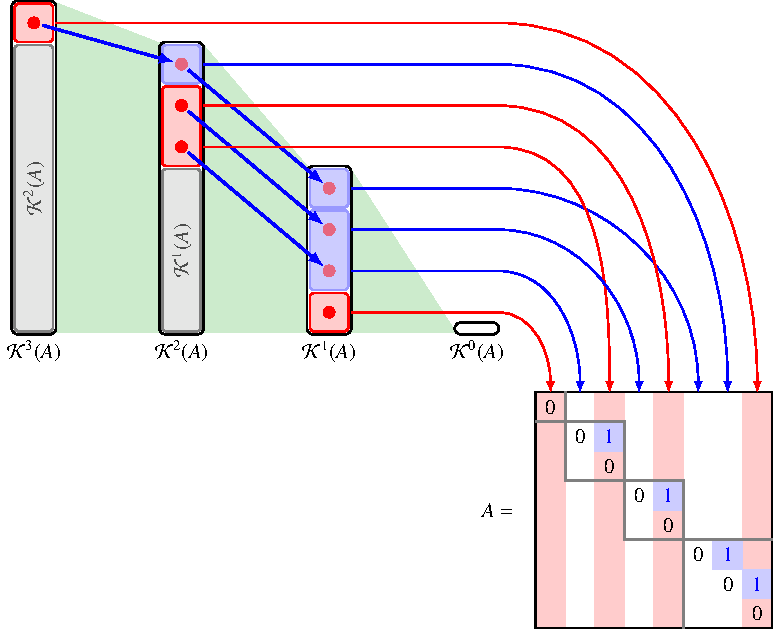
\includegraphics{chapters/40-eigenwerte/images/normalform.pdf}
\caption{Konstruktion der Basis für die Jordansche Normalform einer
nilpotenten Matrix.
Die Vektoren werden in der Reihenfolge von rechts nach links in die
Matrix gefüllt.
\label{buch:eigenwerte:fig:normalform}}
\end{figure}

Abbildung~\ref{buch:eigenwerte:fig:normalform} illustriert den Prozess
an einer nilpotenten Matrix $A$ mit $A^3=0$
Die vertikalen Rechtecke im linken Teil der Abbildung symbolisieren
die Unterräume $\mathcal{K}^k(A)$.
Es ist bekannt, dass $\mathcal{K}^k(A) \subset \mathcal{K}^{k+1}(A)$ ist,
die Einbettung wird in der Abbildung durch graue Rechtecke dargestellt.
Es sei wieder $l$ der Exponent, für den $\mathcal{K}^l(A)=\Bbbk^n$ wird.
Da $\mathcal{K}^{l-1}(A)\ne \mathcal{K}^l(A)$ ist, muss es einen
komplementären Unterraum geben, in dem eine Basis gewählt wird.
Jeder der Vektoren $b_1,\dots,b_s$ dieser Basis gibt Anlass zu einem
Block der Form $N_l$, der auf dem Unterraum 
$\langle b_i,Ab_i,\dots,A^{l-1}b_i\rangle$ operiert.
In der Abbildung ist $b_i$ durch einen roten Punkt symbolisiert und
die Bilder $Ab_i,\dots,A^{l-1}b_i$ werden durch blaue Pfeile untereinander
verbunden.

Der Raum $\mathcal{K}^{l-1}(A)$ enthält dann $\mathcal{K}^{l-2}(A)$ und
die Vektoren $Ab_1,\dots,Ab_s$.
Es ist aber möglich, dass diese Vektoren nicht den ganzen Raum
$\mathcal{K}^{l-1}(A)$ erzeugen.
In diesem Fall lassen sich die Vektoren mit Hilfe weiterer Vektoren
$b_{s+1},\dots,b_{s+r}$ zu einer Basisi von $\mathcal{K}^{l-1}(A)$
ergänzen.
Wie vorhin gibt jeder der Vektoren $b_{s+i}$ Anlass zu einem Block
der Form $N_{l-1}$, der auf dem Unterraum
$\langle b_{s+i},Ab_{s+i}\dots,A^{l-2}b_{s+i}\rangle$
operiert.

Durch Wiederholung dieses Prozesses können schrittweise Basisvektoren
$b_i$ erzeugt werden.
Die Matrix der Abbildung $f$ in der Basis $\{b_i,Ab_i,\dots,A^kb_i\}$
ist ein Block der Form $N_k$.
Für $0\le k\le l-1$ sind die Vektoren $A^kb_i$,
solange sie von $0$ verschieden sind,
alle nach Konstruktion linear unabhängig, sie bilden eine Basis
von $\mathcal{K}^l(A)=\mathbb{R}^n$.

\begin{beispiel}
Die Basis für die Zerlegung der Matrix
\[
A
=
\begin{pmatrix*}[r]
  3& 1&-2\\
-21&-7&14\\
 -6&-2& 4
\end{pmatrix*}
\]
in Blockform soll nach der oben beschriebenen Methode ermittelt werden.
Zunächst kann man nachrechnen, dass $A^2=0$ ist.
Der Kern von $A$ ist der Lösungsraum der Gleichung $Ax=0$, da alle Zeilen
Vielfache der ersten Zeile sind, recht es zu verlangen, dass die
Komponenten $x_i$ der Lösung die Gleichung
\[
3x_1+x_2-2x_3=0
\]
erfüllen.
Jetzt muss ein Vektor $b_1$ ausserhalb von $\mathbb{L}$ gefunden werden,
der erste Standardbasisvektor $e_1$ kann dazu verwendet werden.
Es ist auch klar, dass $Ae_1\ne 0$ ist.
Wir verwenden daher die beiden Vektoren 
\[
b_3=e_1=\begin{pmatrix} 1\\0\\0 \end{pmatrix}
,\qquad
b_2=Ab_3=\begin{pmatrix*}[r] 3\\-21\\-6 \end{pmatrix*},
\]
in dieser Basis hat $A$ die Matrix $N_2$.
Jetzt muss noch ein Basisvektor $b_1$ gefunden werden,
der in $\ker A=\mathbb{L}$ liegt und so, dass $b_1$ und $b_2$ 
linear unabhängig sind.
Die zweite Bedingung kann leicht dadurch sichergestellt werden,
dass man die erste Komponente von $b_1$ als $0$ wählt.
Eine mögliche Lösung ist dann
\[
b_1=\begin{pmatrix}0\\2\\1\end{pmatrix}
\]
Die Matrix 
\[
B=\begin{pmatrix*}[r]
 0& 1&   3\\
 2& 0& -21\\
 1& 0&  -6
\end{pmatrix*}
\qquad\text{mit Inverser}
\qquad
B^{-1}=\begin{pmatrix*}[r]
0&-\frac23& \frac73\\
0&-\frac19& \frac29\\
1& \frac13&-\frac23
\end{pmatrix*}
\]
transformiert die Matrix $A$ auf den Block $N_3$:
\[
B^{-1}AB
=
B^{-1}\begin{pmatrix*}[r]
0&0&  3\\
0&0&-21\\
0&0& -6
\end{pmatrix*}
=
\begin{pmatrix}
0&0&0\\
0&0&1\\
0&0&0
\end{pmatrix}
=
N_3.
\qedhere
\]
\end{beispiel}

%
% Begriff des Eigenwertes und Eigenvektors
%
\subsection{Eigenwerte und Eigenvektoren
\label{buch:subsection:eigenwerte-und-eigenvektoren}}
In diesem Abschnitt betrachten wir Vektorräume $V=\Bbbk^n$ über einem
beliebigen Körper $\Bbbk$ und quadratische Matrizen
$A\in M_n(\Bbbk)$.
In den meisten Anwendungen wird $\Bbbk=\mathbb{R}$ sein.
Da aber in $\mathbb{R}$ nicht alle algebraischen Gleichungen lösbar sind,
ist es manchmal notwendig, den Vektorraum zu erweitern um zum Beispiel
Eigenschaften der Matrix $A$ abzuleiten.

\begin{definition}
Ein Vektor $v\in V$ heisst {\em Eigenvektor} von $A$ zum Eigenwert
$\lambda\in\Bbbk$, wenn $v\ne 0$ und $Av=\lambda v$ gilt.
\end{definition}

Die Bedingung $v\ne 0$ dient dazu, pathologische Situationen auszuschliessen.
Für den Nullvektor gilt $A0=\lambda 0$ für jeden beliebigen Wert von
$\lambda\in\Bbbk$.
Würde man $v=0$ zulassen, wäre jede Zahl in $\Bbbk$ ein Eigenwert,
ein Eigenwert von $A$ wäre nichts besonderes.
Ausserdem wäre $0$ ein Eigenvektor zu jedem beliebigen Eigenwert.

Eigenvektoren sind nicht eindeutig bestimmt, jedes von $0$ verschiedene
Vielfache von $v$ ist ebenfalls ein Eigenvektor.
Zu einem Eigenwert kann man also einen Eigenvektor jeweils mit 
geeigneten Eigenschaften finden, zum Beispiel kann man für $\Bbbk = \mathbb{R}$
Eigenvektoren auf Länge $1$ normieren.
Im Folgenden werden wir oft die abkürzend linear unabhängige Eigenvektoren
einfach als ``verschiedene'' Eigenvektoren bezeichnen.

Wenn $v$ ein Eigenvektor von $A$ zum Eigenwert $\lambda$ ist, dann kann
man ihn mit zusätzlichen Vektoren $v_2,\dots,v_n$ zu einer Basis
$\mathcal{B}=\{v,v_2,\dots,v_n\}$
von $V$ ergänzen.
Die Vektoren $v_k$ mit $k=2,\dots,n$ werden von $A$ natürlich auch
in den Vektorraum $V$ abgebildet, können also als Linearkombinationen
\[
Av = a_{1k}v + a_{2k}v_2 + a_{3k}v_3 + \dots a_{nk}v_n
\]
dargestellt werden.
In der Basis $\mathcal{B}$ bekommt die Matrix $A$ daher die Form
\[
A'
=
\begin{pmatrix}
\lambda&a_{12}&a_{13}&\dots &a_{1n}\\
    0  &a_{22}&a_{23}&\dots &a_{2n}\\
    0  &a_{32}&a_{33}&\dots &a_{3n}\\
\vdots &\vdots&\vdots&\ddots&\vdots\\
    0  &a_{n2}&a_{n3}&\dots &a_{nn}
\end{pmatrix}.
\]
Bereits ein einzelner Eigenwert und ein zugehöriger Eigenvektor
ermöglichen uns also, die Matrix in eine etwas einfachere Form
zu bringen.

\begin{definition}
Für $\lambda\in\Bbbk$ heisst
\[
E_\lambda
=
\{ v\;|\; Av=\lambda v\}
\]
der {\em Eigenraum} zum Eigenwert $\lambda$.
\index{Eigenraum}%
\end{definition}

Der Eigenraum $E_\lambda$ ist ein Unterraum von $V$, denn wenn
$u,v\in E_\lambda$, dann ist
\[
A(su+tv)
=
sAu+tAv
=
s\lambda u + t\lambda v
=
\lambda(su+tv),
\]
also ist auch $su+tv\in E_\lambda$.
Der Fall $E_\lambda = \{0\}=0$ bedeutet natürlich, dass $\lambda$ gar kein
Eigenwert ist.

\begin{satz}
Wenn $\dim E_\lambda=n$, dann ist $A=\lambda E$.
\end{satz}

\begin{proof}[Beweis]
Da $V$ ein $n$-dimensionaler Vektoraum ist, ist $E_\lambda=V$.
Jeder Vektor $v\in V$ erfüllt also die Bedingung $Av=\lambda v$,
oder $A=\lambda E$.
\end{proof}

Wenn man die Eigenräume von $A$ kennt, dann kann man auch die Eigenräume
von $A+\mu E$ berechnen.
Ein Vektor $v\in E_\lambda$ erfüllt
\[
Av=\lambda v
\qquad\Rightarrow\qquad
(A+\mu)v = \lambda v + \mu v
=
(\lambda+\mu)v,
\]
somit ist $v$ ein Eigenvektor von $A+\mu E$ zum Eigenwert $\lambda+\mu$.
Insbesondere können wir statt die Eigenvektoren von $A$ zum Eigenwert $\lambda$
zu studieren, auch die Eigenvektoren zum Eigenwert $0$ von $A-\lambda E$
untersuchen.

%
% Invariante Räume
%
\subsection{Verallgemeinerte Eigenräume
\label{buch:subsection:verallgemeinerte-eigenraeume}}
Wenn $\lambda$ ein Eigenwert der Matrix $A$ ist, dann ist
ist $A-\lambda E$ injektiv und $\ker(A-\lambda E)\ne 0$.
Man kann daher die invarianten Unterräume $\mathcal{K}(A-\lambda E)$
und $\mathcal{J}(A-\lambda E)$.

\begin{beispiel}
Wir untersuchen die Matrix
\[
A
=
\begin{pmatrix}
1&1&-1&0\\
0&3&-1&1\\
0&2& 0&1\\
0&0& 0&2
\end{pmatrix}
\]
Man kann zeigen, dass $\lambda=1$ ein Eigenwert ist.
Wir suchen die Zerlegung des Vektorraums $\mathbb{R}^4$ in invariante
Unterräume $\mathcal{K}(A-E)$ und $\mathcal{J}(A-E)$.
Die Matrix $B=A-E$ ist
\[
B
=
\begin{pmatrix}
0&1&-1&0\\
0&2&-1&1\\
0&2&-1&1\\
0&0& 0&2
\end{pmatrix}
\]
und wir berechnen davon die Potenz
\[
D=B^4=(A-E)^4
=
\begin{pmatrix}
0&0& 0&0\\
0&2&-1&4\\
0&2&-1&4\\
0&0& 0&1
\end{pmatrix}.
\]
Daraus kann man ablesen, dass das Bild $\operatorname{im}D$
von $D$ die Basis
\[
b_1
=
\begin{pmatrix}
0\\0\\0\\1
\end{pmatrix}
, \qquad
b_2
=
\begin{pmatrix}
0\\1\\1\\0
\end{pmatrix}
\]
hat.
Für den Kern von $D$ können wir zum Beispiel die Basisvektoren
\[
b_3
=
\begin{pmatrix}
0\\1\\2\\0
\end{pmatrix}
,\qquad
b_4
=
\begin{pmatrix}
1\\0\\0\\0
\end{pmatrix}
\]
verwenden.

Als erstes überprüfen wir, ob diese Basisvektoren tatsächlich invariante
Unterräume sind.
Für $\mathcal{J}(A-E) = \langle b_1,b_2\rangle$
berechnen wir
\begin{align*}
(A-E)b_1
&=
\begin{pmatrix} 0\\4\\4\\1 \end{pmatrix}
=
4b_2+b_1,
\\
(A-E)b_2
&=
\begin{pmatrix} 0\\1\\1\\0 \end{pmatrix}
=
b_2.
\end{align*}
Dies beweist, dass $\mathcal{J}(A-E)$ invariant ist.
In dieser Basis hat die von $A-E$ beschriebene lineare Abbildung
auf $\mathcal{J}(A-E)$ die Matrix
\[
A_{\mathcal{J}(A-E)}
=
\begin{pmatrix}
1&4\\
0&1
\end{pmatrix}.
\]

Für den Kern $\mathcal{K}(A-E)$ findet man analog
\[
\left.
\begin{aligned}
Ab_3
&=
-b_4
\\
Ab_4
&=0
\end{aligned}
\quad\right\}
\qquad\Rightarrow\qquad
A_{\mathcal{K}(A-E)}
=
\begin{pmatrix}
0&-1\\
0& 0
\end{pmatrix}.
\]
In der Basis $\mathcal{B}=\{b_1,b_2,b_3,b_4\}$ hat $A$ die Matrix
in Blockform
\[
A'
=
\left(
\begin{array}{cc|cr}
2&4& & \\
0&2& & \\
\hline
 & &1&-1\\
 & &0& 1
\end{array}\right),
\]
die Blöcke gehören zu den invarianten Unterräumen $\mathcal{K}(A-E)$
und $\mathcal{K}(A-E)$.
Die aus $A-E$ gewonnen invarianten Unterräume sind offenbar auch invariante
Unterräume für $A$.
\end{beispiel}

\begin{definition}
Ist $A$ eine Matrix mit Eigenwert $\lambda$, dann heisst der invariante
Unterraum
\[
\mathcal{E}_{\lambda}(A)
=
\mathcal{K}(A-\lambda E)
\]
der verallgemeinerte Eigenraum von $A$.
\end{definition}

Es ist klar, dass
$E_\lambda(A)=\ker (A-\lambda E)\subset\mathcal{E}_{\lambda}(A)$.

\subsection{Zerlegung in invariante Unterräume
\label{buch:subsection:zerlegung-in-invariante-unterraeume}}
Wenn $\lambda$ kein Eigenwert von $A$ ist, dann ist $A-\lambda E$
injektiv und damit $\ker(A-\lambda E)=0$.
Es folgt, dass $\mathcal{K}^i(A-\lambda E)=0$ und daher auch
$\mathcal{J}^i(A-\lambda E)=V$.
Die Zerlegung in invariante Unterräume $\mathcal{J}(A-\lambda E)$ und
$\mathcal{K}(A-\lambda E)$ liefert in diesem Falle also nichts Neues.

Für einen Eigenwert $\lambda_1$ von $A$ dagegen, erhalten wir die Zerlegung
\[
V
=
\mathcal{E}_{\lambda_1}(A)
\oplus
\underbrace{\mathcal{J}(A-\lambda_1 E)}_{\displaystyle =V_2},
\]
wobei $\mathcal{E}_{\lambda_1}(A)\ne 0$ ist.
Die Matrix $A-\lambda_1 E$ ist eingeschränkt auf $\mathcal{E}_{\lambda_1}(A)$
nilpotent.
Die Zerlegung in invariante Unterräume ist zwar mit Hilfe von $A-\lambda_1E$
gewonnen worden, ist aber natürlich auch eine Zerlegung in invariante 
Unterräume für $A$.
Wir können daher das Problem auf $V_2$ einschränken und nach einem weiteren
Eigenwert $\lambda_2$ von $A$ in $V_2$ suchen, was wieder eine Zerlegung
in invariante Unterräume liefert.
Indem wir so weiterarbeiten, bis wir den ganzen Raum ausgeschöpft haben,
können wir eine Zerlegung des ganzen Raumes $V$ finden, so dass $A$ auf
jedem einzelnen Summanden eine sehr einfach Form hat:

\begin{satz}
\label{buch:eigenwerte:satz:zerlegung-in-eigenraeume}
Sei $V$ ein $\Bbbk$-Vektorraum und $f$ eine lineare Abbildung mit Matrix
$A$ derart, dass alle Eigenwerte $\lambda_1,\dots,\lambda_l$ von $A$
in $\Bbbk$ sind.
Dann gibt es eine Zerlegung von $V$ in verallgemeinerte Eigenräume
\[
V
=
\mathcal{E}_{\lambda_1}(A)
\oplus
\mathcal{E}_{\lambda_2}(A)
\oplus
\dots
\oplus
\mathcal{E}_{\lambda_l}(A).
\]
Die Einschränkung von $A-\lambda_{i}E$ auf den Eigenraum 
$\mathcal{E}_{\lambda_i}(A)$ ist nilpotent.
\end{satz}

\subsection{Das charakteristische Polynom
\label{buch:subsection:das-charakteristische-polynom}}
Ein Eigenvektor von $A$ erfüllt $Av=\lambda v$ oder gleichbedeutend
$(A-\lambda E)v=0$, er ist also eine nichttriviale Lösung des homogenen
Gleichungssystems mit Koeffizientenmatrix $A-\lambda E$. 
Ein Eigenwert ist also ein Skalar derart, dass $A-\lambda E$
singulär ist.
Ob eine Matrix singulär ist, kann mit der Determinante festgestellt
werden.
Die Eigenwerte einer Matrix $A$ sind daher die Nullstellen
von $\det(A-\lambda E)$.

\begin{definition}
Das {\em charakteristische Polynom}
\[
\chi_A(x)
=
\det (A-x E)
=
\left|
\begin{matrix}
a_{11}-x & a_{12}   & \dots  & a_{1n} \\
a_{21}   & a_{22}-x & \dots  & a_{2n} \\
\vdots   &\vdots    &\ddots  & \vdots \\
a_{n1}   & a_{n2}   &\dots   & a_{nn}-x
\end{matrix}
\right|.
\]
der Matrix $A$ ist ein Polynom vom Grad $n$ mit Koeffizienten in $\Bbbk$.
\end{definition}

Findet man eine Nullstelle $\lambda\in\Bbbk$ von $\chi_A(x)$,
dann ist die Matrix $A-\lambda E\in M_n(\Bbbk)$ und mit dem Gauss-Algorithmus
kann man auch mindestens einen Vektor $v\in \Bbbk^n$ finden,
der $Av=\lambda v$ erfüllt.
Eine Matrix der Form  wie in Satz~\ref{buch:eigenwerte:satz:jordanblock}
hat
\[
\chi_A(x)
=
\left|
\begin{matrix}
\lambda-x &     1     &           &      &         &         \\
          & \lambda-x &     1     &      &         &         \\
          &           & \lambda-x &      &         &         \\
          &           &           &\ddots&         &         \\
          &           &           &      &\lambda-x&     1   \\
          &           &           &      &         &\lambda-x
\end{matrix}
\right|
=
(\lambda-x)^n
=
(-1)^n (x-\lambda)^n
\]
als charakteristisches Polynom, welches $\lambda$ als einzige
Nullstelle hat.
Der Eigenraum der Matrix ist aber nur eindimensional, man kann also
im Allgemeinen für jede Nullstelle des charakteristischen Polynoms
nicht mehr als einen Eigenvektor (d.~h.~einen eindimensionalen Eigenraum)
erwarten.

Wenn das charakteristische Polynom von $A$ keine Nullstellen in $\Bbbk$ hat,
dann kann es auch keine Eigenvektoren in $\Bbbk^n$ geben.
Gäbe es nämlich einen solchen Vektor, dann müsste eine der Komponenten
des Vektors von $0$ verschieden sein, wir nehmen an, dass es die Komponente
in Zeile $k$ ist.
Die Komponente $v_k$ kann man auf zwei Arten berechnen, einmal als
die $k$-Komponenten von $Av$ und einmal als $k$-Komponente von $\lambda v$:
\[
a_{k1}v_1+\dots+a_{kn}v_n = \lambda v_k.
\]
Da $v_k\ne 0$ kann man nach $\lambda$ auflösen und erhält
\[
\lambda = \frac{a_{k1}v_1+\dots + a_{kn}v_n}{v_k}.
\]
Alle Terme auf der rechten Seite sind in $\Bbbk$ und werden nur mit
Körperoperationen in $\Bbbk$ verknüpft, also muss auch $\lambda\in\Bbbk$
sein, im Widerspruch zur Annahme.

Durch Hinzufügen von geeigneten Elementen können wir immer zu einem 
Körper $\Bbbk'$ übergehen, in dem das charakteristische Polynom
in Linearfaktoren zerfällt.
In diesem Körper kann man jetzt das homogene lineare Gleichungssystem
mit Koeffizientenmatrix $A-\lambda E$ lösen und damit mindestens 
einen Eigenvektor $v$ für jeden Eigenwert finden.
Die Komponenten von $v$ liegen in $\Bbbk'$, und mindestens eine davon kann
nicht in $\Bbbk$ liegen.
Das bedeutet aber nicht, dass man diese Vektoren nicht für theoretische
Überlegungen über von $\Bbbk'$ unabhängige Eigenschaften der Matrix $A$ machen.
Das folgende Beispiel soll diese Idee illustrieren.

\begin{beispiel}
Wir arbeiten in diesem Beispiel über dem Körper $\Bbbk=\mathbb{Q}$.
Die Matrix
\[
A=\begin{pmatrix}
-4&7\\
-2&4
\end{pmatrix}
\in
M_2(\mathbb{Q})
\]
hat das charakteristische Polynom
\[
\chi_A(x)
=
\left|
\begin{matrix}
-4-x&7\\-2&4-x
\end{matrix}
\right|
=
(-4-x)(4-x)-7\cdot(-2)
=
-16+x^2+14
=
x^2-2.
\]
Die Nullstellen sind $\pm\sqrt{2}$ und damit nicht in $\mathbb{Q}$.
Wir gehen daher über zum Körper $\mathbb{Q}(\!\sqrt{2})$, in dem
sich zwei Nullstellen $\lambda=\pm\sqrt{2}$ finden lassen.
Zu jedem Eigenwert lässt sich auch ein Eigenvektor
$v_{\pm\sqrt{2}}\in \mathbb{Q}(\!\sqrt{2})^2$, und unter Verwendung dieser
Basis bekommt die Matrix $A'=TAT^{-1}$ Diagonalform.
Die Transformationsmatrix $T$ enthält Matrixelemente aus
$\mathbb{Q}(\!\sqrt{2})$, die nicht in $\mathbb{Q}$ liegen.
Die Matrix $A$ lässt sich also über dem Körper $\mathbb{Q}(\!\sqrt{2})$
diagonalisieren, nicht aber über dem Körper $\mathbb{Q}$.

Da $A'$ Diagonalform hat mit $\pm\sqrt{2}$ auf der Diagonalen, folgt
$A^{\prime 2} = 2E$, die Matrix $A'$ erfüllt also die Gleichung
\begin{equation}
A^{\prime 2}-E= \chi_{A}(A) = 0.
\label{buch:grundlagen:eqn:cayley-hamilton-beispiel}
\end{equation}
Dies is ein Spezialfall des Satzes von Cayley-Hamilton~\ref{XXX}
welcher besagt, dass jede Matrix $A$ eine Nullstelle ihres 
charakteristischen Polynoms ist: $\chi_A(A)=0$.
Die Gleichung~\ref{buch:grundlagen:eqn:cayley-hamilton-beispiel}
wurde zwar in $\mathbb{Q}(\!\sqrt{2})$ hergeleitet, aber in ihr kommen
keine Koeffizienten aus $\mathbb{Q}(\!\sqrt{2})$ vor, die man nicht auch
in $\mathbb{Q}$ berechnen könnte.
Sie gilt daher ganz allgemein.
\end{beispiel}

\begin{beispiel}
Die Matrix
\[
A=\begin{pmatrix}
32&-41\\
24&-32
\end{pmatrix}
\in
M_2(\mathbb{R})
\]
über dem Körper $\Bbbk = \mathbb{R}$
hat das charakteristische Polynom
\[
\det(A-xE)
=
\left|
\begin{matrix}
32-x&-41  \\
25  &-32-x
\end{matrix}
\right|
=
(32-x)(-32-x)-25\cdot(-41)
=
x^2-32^2 + 1025
=
x^2+1.
\]
Die charakteristische Gleichung $\chi_A(x)=0$ hat in $\mathbb{R}$
keine Lösungen, daher gehen wir zum Körper $\Bbbk'=\mathbb{C}$ über,
in dem dank dem Fundamentalsatz der Algebra alle Nullstellen zu finden
sind, sie sind $\pm i$.
In $\mathbb C$ lassen sich dann auch Eigenvektoren finden, man muss dazu die
folgenden linearen Gleichungssyteme lösen:
\begin{align*}
\begin{tabular}{|>{$}c<{$}>{$}c<{$}|}
32-i&-41\\
25  &-32-i
\end{tabular}
&
\rightarrow
\begin{tabular}{|>{$}c<{$}>{$}c<{$}|}
1 & t\\
0 &  0 
\end{tabular}
&
\begin{tabular}{|>{$}c<{$}>{$}c<{$}|}
32+i&-41\\
25  &-32+i
\end{tabular}
&
\rightarrow
\begin{tabular}{|>{$}c<{$}>{$}c<{$}|}
1 & \overline{t}\\
0 &  0 
\end{tabular},
\intertext{wobei wir $t=-41/(32-i) =-41(32+i)/1025= -1.28 -0.04i = (64-1)/50$
abgekürzt haben.
Die zugehörigen Eigenvektoren sind}
v_i&=\begin{pmatrix}t\\i\end{pmatrix}
&
v_{-i}&=\begin{pmatrix}\overline{t}\\i\end{pmatrix}
\end{align*}
Mit den Vektoren $v_i$ und $v_{-i}$ als Basis kann die Matrix $A$ als
komplexe Matrix, also mit komplexem $T$ in die komplexe Diagonalmatrix 
$A'=\operatorname{diag}(i,-i)$ transformiert werden.
Wieder kann man sofort ablesen, dass $A^{\prime2}+E=0$, und wieder kann
man schliessen, dass für die relle Matrix $A$ ebenfalls $\chi_A(A)=0$
gelten muss.
\end{beispiel}





%
% normalformen.tex -- Normalformen einer Matrix
%
% (c) 2021 Prof Dr Andreas Müller, OST Ostschweizer Fachhochschule
%
\section{Normalformen
\label{buch:section:normalformen}}
\rhead{Normalformen}
In den Beispielen im vorangegangenen wurde wiederholt der Trick
verwendet, den Koeffizientenkörper so zu erweitern, dass das
charakteristische Polynom in Linearfaktoren zerfällt und 
für jeden Eigenwert Eigenvektoren gefunden werden können.
Diese Idee ermöglicht, eine Matrix in einer geeigneten Körpererweiterung
in eine besonders einfache Form zu bringen, das Problem dort zu lösen.
Anschliessend kann man sich darum kümmern in welchem Mass die gewonnenen
Resultate wieder in den ursprünglichen Körper transportiert werden können.

\subsection{Diagonalform}
Sei $A$ eine beliebige Matrix mit Koeffizienten in $\Bbbk$ und sei $\Bbbk'$
eine Körpererweiterung von $\Bbbk$ derart, dass das charakteristische
Polynom in Linearfaktoren
\[
\chi_A(x)
=
(x-\lambda_1)^{k_1}\cdot (x-\lambda_2)^{k_2}\cdot\dots\cdot (x-\lambda_m)^{k_m}
\]
mit Vielfachheiten $k_1$ bis $k_m$ zerfällt, $\lambda_i\in\Bbbk'$.
Zu jedem Eigenwert $\lambda_i$ gibt es sicher einen Eigenvektor, wir 
wollen aber in diesem Abschnitt zusätzlich annehmen, dass es eine Basis
aus Eigenvektoren gibt.
In dieser Basis bekommt die Matrix Diagonalform, wobei auf der 
Diagonalen nur Eigenwerte vorkommen können.
Man kann die Vektoren so anordnen, dass die Diagonalmatrix in Blöcke
der Form $\lambda_iE$ zerfällt
\[
\def\temp#1{\multicolumn{1}{|c}{\raisebox{0pt}[12pt][7pt]{\phantom{x}$#1$}\phantom{x}}}
A'
=\left(
\begin{array}{cccc}
\cline{1-1}
\temp{\lambda_1E} &\multicolumn{1}{|c}{}&        &           \\
\cline{1-2}
          &\temp{\lambda_2E}&\multicolumn{1}{|c}{}&           \\
\cline{2-3}
          &           &\temp{\ddots}&\multicolumn{1}{|c}{}\\
\cline{3-4}
          &           &        &\multicolumn{1}{|c|}{\raisebox{0pt}[12pt][7pt]{\phantom{x}$\lambda_mE$}\phantom{x}}\\
\cline{4-4}
\end{array}
\right)
\]
Über die Grösse eines solchen $\lambda_iE$-Blockes können wir zum jetzigen
Zeitpunkt noch keine Aussagen machen.

Die Matrizen $A-\lambda_kE$ enthalten jeweils einen Block aus lauter
Nullen.
Das Produkt all dieser Matrizen  ist daher
\[
(A-\lambda_1E)
(A-\lambda_2E)
\cdots
(A-\lambda_mE)
=
0.
\]
Über dem Körper $\Bbbk'$ gibt es also das Polynom
$m(x)=(x-\lambda_1)(x-\lambda_2)\cdots(x-\lambda_m)$ mit der Eigenschaft
$m(A)=0$.
Dies ist auch das Polynom von kleinstmöglichem Grad, denn für jeden
Eigenwert muss ein entsprechender Linearfaktor in so einem Polynom vorkommen.
Das Polynom $m(x)$ ist daher das Minimalpolynom der Matrix $A$.
Da jeder Faktor in $m(x)$ auch ein Faktor von $\chi_A(x)$ ist,
folgt wieder $\chi_A(A)=0$.
Ausserdem ist über dem Körper $\Bbbk'$ das Polynom $m(x)$ ein Teiler
des charakteristischen Polynoms $\chi_A(x)$.

\subsection{Jordan-Normalform
\label{buch:subsection:jordan-normalform}}
Die Eigenwerte einer Matrix $A$ können als Nullstellen des 
charakteristischen Polynoms gefunden werden.
Da der Körper $\Bbbk$ nicht unbedingt algebraische abgeschlossen ist,
zerfällt das charakteristische Polynom nicht unbedingt in Linearfaktoren,
die Nullstellen sind nicht unbedingt in $\Bbbk$.
Wir können aber immer zu einem grösseren Körper $\Bbbk'$ übergehen,
in dem das charakteristische Polynom in Linearfaktoren zerfällt.
Wir nehmen im Folgenden an, dass 
\[
\chi_A(x)
=
(x-\lambda_1)^{k_1}
\cdot
(x-\lambda_2)^{k_2}
\cdot
\dots
\cdot
(x-\lambda_l)^{k_l}
\]
ist mit $\lambda_i\in\Bbbk'$.

Nach Satz~\ref{buch:eigenwerte:satz:zerlegung-in-eigenraeume} liefern
die verallgemeinerten Eigenräume $V_i=\mathcal{E}_{\lambda_i}(A)$ eine
Zerlegung von $V$ in invariante Eigenräume
\[
V=V_1\oplus V_2\oplus \dots\oplus V_l,
\]
derart, dass $A-\lambda_iE$ auf $V_i$ nilpotent ist.
Wählt man in jedem der Unterräume $V_i$ eine Basis, dann zerfällt die
Matrix $A$ in Blockmatrizen
\begin{equation}
\def\temp#1{\multicolumn{1}{|c}{\raisebox{0pt}[17pt][12pt]{\phantom{x}$#1\mathstrut$}\phantom{x}}}
A'
=\left(
\begin{array}{cccc}
\cline{1-1}
\temp{A_{1}} &\multicolumn{1}{|c}{}&        &           \\
\cline{1-2}
          &\temp{A_{2}}&\multicolumn{1}{|c}{}&           \\
\cline{2-3}
          &           &\temp{\ddots}&\multicolumn{1}{|c}{}\\
\cline{3-4}
          &           &        &\multicolumn{1}{|c|}{\raisebox{0pt}[17pt][12pt]{\phantom{x}$A_{l}$}\phantom{x}}\\
\cline{4-4}
\end{array}
\right)
\label{buch:eigenwerte:eqn:allgnilpotent}
\end{equation}
wobei, $A_i$ Matrizen mit dem einzigen Eigenwert $\lambda_i$ sind.

Nach Satz~\ref{buch:eigenwerte:satz:allgnilpotent}
kann man in den Unterräume die Basis zusätzlich so wählen, dass 
die entstehenden Blöcke $A_i-\lambda_i E$ spezielle nilpotente Matrizen
aus lauter Null sind, die höchstens unmittelbar über der Diagonalen
Einträge $1$ haben kann.
Dies bedeutet, dass sich immer eine Basis so wählen lässt, dass die
Matrix $A_i$ zerfällt in sogenannte Jordan-Blöcke.

\begin{definition}
Ein $m$-dimensionaler {\em Jordan-Block} ist eine $m\times m$-Matrix
\index{Jordan-Block}%
der Form
\[
J_m(\lambda)
=
\begin{pmatrix}
\lambda &    1    &         &        &         &         \\
        & \lambda &    1    &        &         &         \\
        &         & \lambda &        &         &         \\
        &         &         & \ddots &         &         \\
        &         &         &        & \lambda &     1   \\
        &         &         &        &         & \lambda 
\end{pmatrix}.
\]
Eine {\em Jordan-Matrix} ist eine Blockmatrix Matrix
\[
J
=
\def\temp#1{\multicolumn{1}{|c}{\raisebox{0pt}[17pt][12pt]{\phantom{x}$#1\mathstrut$}\phantom{x}}}
\left(
\begin{array}{cccc}
\cline{1-1}
\temp{J_{m_1}(\lambda)} &\multicolumn{1}{|c}{}&        &           \\
\cline{1-2}
          &\temp{J_{m_2}(\lambda)}&\multicolumn{1}{|c}{}&           \\
\cline{2-3}
          &           &\temp{\ddots}&\multicolumn{1}{|c}{}\\
\cline{3-4}
          &           &        &\multicolumn{1}{|c|}{\raisebox{0pt}[17pt][12pt]{\phantom{x}$J_{m_p}(\lambda)$}\phantom{x}}\\
\cline{4-4}
\end{array}
\right)
\]
mit $m_1+m_2+\dots+m_p=m$.
\index{Jordan-Matrix}%
\end{definition}

Da Jordan-Blöcke obere Dreiecksmatrizen sind, ist
das charakteristische Polynom eines Jordan-Blocks oder einer Jordan-Matrix
besonders einfach zu berechnen.
Es gilt
\[
\chi_{J_m(\lambda)}(x)
=
\det (J_m(\lambda) - xE)
=
(\lambda-x)^m
\]
für einen Jordan-Block $J_m(\lambda)$.
Für eine $m\times m$-Jordan-Matrix $J$ mit Blöcken $J_{m_1}(\lambda)$
bis $J_{m_p}(\lambda)$ ist
\[
\chi_{J(\lambda)}(x)
=
\chi_{J_{m_1}(\lambda)}(x)
\chi_{J_{m_2}(\lambda)}(x)
\cdot
\dots
\cdot
\chi_{J_{m_p}(\lambda)}(x)
=
(\lambda-x)^{m_1}
(\lambda-x)^{m_2}
\cdot\dots\cdot
(\lambda-x)^{m_p}
=
(\lambda-x)^m.
\]

\begin{satz}
\label{buch:eigenwerte:satz:jordannormalform}
Über einem Körper $\Bbbk'\supset\Bbbk$, über dem das charakteristische
Polynom $\chi_A(x)$ in Linearfaktoren zerfällt, lässt sich immer
eine Basis finden derart, dass die Matrix $A$ zu einer Blockmatrix wird,
die aus lauter Jordan-Matrizen besteht.
Die Dimension der Jordan-Matrix zum Eigenwert $\lambda_i$ ist die
Vielfachheit des Eigenwerts im charakteristischen Polynom.
\end{satz}

\begin{proof}[Beweis]
Es ist nur noch die Aussage über die Dimension der Jordan-Blöcke zu
beweisen.
Die Jordan-Matrizen zum Eigenwert $\lambda_i$ werden mit $J_i$
bezeichnet und sollen $m_i\times m_i$-Matrizen sein.
Das charakteristische Polynom jedes Jordan-Blocks ist dann
$\chi_{J_i}(x)=(\lambda_i-x)^{m_i}$.
Das charakteristische Polynom der Blockmatrix mit diesen Jordan-Matrizen
als Blöcken ist das Produkt
\[
\chi_A(x)
=
(\lambda_1-x)^{m_1}
(\lambda_2-x)^{m_2}
\cdots
(\lambda_p-x)^{m_p}
\]
mit $m_1+m_2+\dots+m_p$.
Die Blockgrösse $m_i$ ist also auch die Vielfachheit von $\lambda_i$ im
charakteristischen Polynom $\chi_A(x)$.
\end{proof}



\begin{satz}[Cayley-Hamilton]
Ist $A$ eine $n\times n$-Matrix über dem Körper $\Bbbk$, dann gilt
$\chi_A(A)=0$.
\end{satz}

\begin{proof}[Beweis]
Zunächst gehen wir über zu einem Körper $\Bbbk'\supset\Bbbk$, indem
das charakteristische Polynom $\chi_A(x)$ in Linearfaktoren
$\chi_A(x)
=
(\lambda_1-x)^{m_1}
(\lambda_2-x)^{m_2}
\dots
(\lambda_p-x)^{m_p}$
zerfällt.
Im Vektorraum $\Bbbk'$ kann man eine Basis finden, in der die Matrix
$A$ in Jordan-Matrizen $J_1,\dots,J_p$ zerfällt, wobei $J_i$ eine
$m_i\times m_i$-Matrix ist.
Für den Block mit der Nummer $i$ erhalten wir
$(J_i - \lambda_i E)^{m_i} = 0$.
Setzt man also den Block $J_i$ in das charakteristische Polynom
$\chi_A(x)$ ein, erhält man
\[
\chi_A(J_i)
=
(\lambda_1E - J_1)^{m_1}
\cdot
\ldots
\cdot
\underbrace{
(\lambda_iE - J_i)^{m_i}
}_{\displaystyle=0}
\cdot
\ldots
\cdot
(\lambda_iE - J_p)^{m_p}
=
0.
\]
Jeder einzelne Block $J_i$ wird also zu $0$, wenn man ihn in das
charakteristische Polynome $\chi_A(x)$ einsetzt.
Folglich gilt auch $\chi_A(A)=0$.

Die Rechnung hat zwar im Körper $\Bbbk'$ stattgefunden, aber die Berechnung
$\chi_A(A)$ kann in $\Bbbk$ ausgeführt werden, also ist $\chi_A(A)=0$.
\end{proof}

Aus dem Beweis kann man auch noch eine strengere Bedingung ableiten.
Auf jedem verallgemeinerten Eigenraum $\mathcal{E}_{\lambda_i}(A)$
ist $A_i-\lambda_i$ nilpotent, es gibt also einen minimalen Exponenten
$q_i$ derart, dass $(A_i-\lambda_iE)^{q_i}=0$ ist.
Wählt man eine Basis in jedem verallgemeinerten Eigenraum derart,
dass $A_i$ eine Jordan-Matrix ist, kann man wieder zeigen, dass
für das Polynom
\[
m_A(x)
=
(x-\lambda_1x)^{q_1}
(x-\lambda_2x)^{q_2}
\cdot
\ldots
\cdot
(x-\lambda_px)^{q_p}
\]
gilt $m_A(A)=0$.
$m_A(x)$ ist das {\em Minimalpolynom} der Matrix $A$.
\index{Minimalpolynom einer Matrix}%

\begin{satz}[Minimalpolynom]
Über dem Körper $\Bbbk'\subset\Bbbk$, über dem das charakteristische
Polynom $\chi_A(x)$ in Linearfaktoren zerfällt, ist das Minimalpolynom
von $A$ das Polynom
\[
m(x)
=
(x-\lambda_1)^{q_1}
(x-\lambda_2)^{q_2}
\cdots
\ldots
\cdots
(x-\lambda_p)^{q_p}
\]
wobei $q_i$ der kleinste Index ist, für den die $q_i$-te Potenz
derEinschränkung von $A-\lambda_i E$ auf den verallgemeinerten Eigenraum
$\mathcal{E}_{\lambda_i}(A)$ verschwindet.
Es ist das Polynom geringsten Grades über $\Bbbk'$, welches $m(A)=0$ erfüllt.
\end{satz}


\subsection{Reelle Normalform
\label{buch:subsection:reelle-normalform}}

\subsection{Obere Hessenberg-Form
\label{buch:subsection:obere-hessenberg-form}}




%
% spektralradius.tex
%
% (c) 2020 Prof Dr Andreas Müller, Hochschule Rapperswi
%
\section{Analytische Funktionen einer Matrix
\label{buch:section:analytische-funktionen-einer-matrix}}
\rhead{Analytische Funktionen einer Matrix}
Eine zentrale Motivation in der Entwicklung der Eigenwerttheorie
war das Bestreben, Potenzen $A^k$ auch für grosse $k$ effizient
zu berechnen.
Mit der Jordan-Normalform ist dies auch gelungen, wenigstens über
einem Körper, in dem das charakteristische Polynom in Linearfaktoren
zerfällt.
Die Berechnung von Potenzen war aber nur der erste Schritt, das Ziel
in diesem Abschnitt ist, $f(A)$ für eine genügend grosse Klasse von
Funktionen $f$ berechnen zu können.

%
% Polynom-Funktionen von Matrizen
%
\subsection{Polynom-Funktionen
\label{buch:subsection:polynom-funktionen}}
In diesem Abschnitt ist $B\in M_n(\Bbbk)$ und $\Bbbk'\supset\Bbbk$ ein
Körper, über dem das charakteristische Polynome $\chi_A(x)$ in
Linearfaktoren
\[
\chi_A(x)
=
(\lambda_1-x)^{m_1}(\lambda_2-x)^{m_2}\cdot\ldots\cdot(\lambda_p-x)^{m_p}
\]
zerfällt.

Für jedes beliebige Polynome $p(X)\in\Bbbk[X]$ der Form
\[
p(X) = a_nX^n + a_{n-1}X^{n-1} + \dots a_1x + a_0
\]
kann man auch
\[
p(A) = a_nA^n + a_{n-1}A^{n-1} + \dots a_1A + a_0E
\]
berechnen.
In der Jordan-Normalform können die Potenzen $A^k$ leicht zusammengstellt
werden, sobald man die Potenzen von Jordan-Blöcken berechnet hat.

\begin{satz}
Die $k$-te Potenz von $J_n(\lambda)$ ist die Matrix mit
\begin{equation}
J_n(\lambda)^k
=
\begin{pmatrix}
\lambda^k
	& \binom{k}{1}\lambda^{k-1}
		& \binom{k}{2} \lambda^{k-2}
			& \binom{k}{3} \lambda^{k-3}
				& \dots
					&\binom{k}{n-1}\lambda^{k-n+1}
\\
0
	& \lambda^k
		& \binom{k}{1}\lambda^{k-1}
			& \binom{k}{2} \lambda^{k-2}
				& \dots
					&\binom{k}{n-2}\lambda^{k-n+2}
\\
0
	& 0
		& \lambda^k
			& \binom{k}{1}\lambda^{k-1}
				& \dots
					&\binom{k}{n-3}\lambda^{k-n+3}
\\
\vdots  &\vdots &\vdots &\vdots &\ddots & \vdots
\\
0	& 0	& 0	& 0	& \dots	& \lambda^k
\end{pmatrix}
\label{buch:eigenwerte:eqn:Jnkpotenz}
\end{equation}
mit den Matrixelementen
\[
(J_n(\lambda)^k)_{ij}
=
\binom{k}{j-i}\lambda^{k-j+i}.
\]
Die Binomialkoeffizienten verschwinden für $j<i$ und $j>i+k$.
\end{satz}

\begin{proof}[Beweis]
Die Herkunft der Binomialkoeffizienten wird klar, wenn man
\[
J_n(\lambda) = \lambda E + N_n
\]
schreibt, wobei $N_n$ die Matrix \eqref{buch:eigenwerte:eqn:nnilpotent} ist.
Die Potenzen von $N_n$ haben die Matrix-Elemente
\[
(N_n^k)_{ij}
=
\delta_{i,j-k}
=
\begin{cases}
1&\qquad j-i=k\\
0&\qquad\text{sonst,}
\end{cases}
\]
sie haben also Einsen genau dort, wo in der
\label{buch:eigenwerte:eqn:Jnkpotenz} die Potenz $\lambda^{k}$ steht.
Die $kt$-te Potenz von $J_n(\lambda)$ kann dann mit dem binomischen
Satz berechnet werden:
\[
J_n(\lambda)^k
=
\sum_{l=0}^k \binom{k}{l}\lambda^l N_n^{k-l},
\]
dies ist genau die Form \eqref{buch:eigenwerte:eqn:Jnkpotenz}.
\end{proof}

Wir haben bereits gesehen, dass $\chi_A(A)=0$, ersetzt man also das
Polynom $p(X)$ durch $p(X)+\chi_A(X)$, dann ändert sich am Wert 
\[
(p+\chi_A)(A)
=
p(A) + \chi_A(A)
=
p(A)
\]
nichts.
Man kann also nicht erwarten, dass verschiedene Polynome 
$p(X)$ zu verschiedenen Matrizen $p(A)$ führen.
Doch welche Unterschiede zwischen Polynomen wirken sich genau aus?

\begin{satz}
Für zwei Polynome $p(X)$ und $q(X)$ ist genau dann $p(A)=q(A)$, wenn
das Minimalpolynom von $A$ die Differenz $p-q$ teilt.
\end{satz}

\begin{proof}[Beweis]
Wenn $p(A)=q(A)$, dann ist $h(X)=p(X)-q(X)$ ein Polynom mit $h(A)=0$,
daher muss $h(X)$ vom Minimalpolynom geteilt werden.
Ist andererseits $p(X)-q(X)=m(X)t(X)$, dann ist
$p(A)-q(A)=m(A)t(A)=0\cdot t(A) = 0$, also $p(A)=q(A)$.
\end{proof}

Über einem Körper $\Bbbk'\supset\Bbbk$, über dem das charakteristische
Polynom in Linearfaktoren zerfällt, kann man das Minimalpolynom aus
der Jordanschen Normalform ableiten.
Es ist
\[
m(X)
=
(\lambda_1-X)^{q_1}
(\lambda_2-X)^{q_2}
\cdot\ldots
\cdot
(\lambda_p-X)^{q_p},
\]
wobei $q_i$ die Dimension des grössten Jordan-Blocks ist, der in der
Jordan-Normalform vorkommt.
Zwei Polynome $p_1(X)$ und $p_2(X)$ haben genau dann den gleichen Wert,
wenn die Differenz $p_1(X)-p_2(X)$ genau die Nullstellen
$\lambda_1,\dots,\lambda_p$ mit Vielfachheiten $q_1,\dots,q_p$ hat.

\begin{beispiel}
Wir betrachten die Matrix
\[
A
=
\begin{pmatrix}
   1&  9& -4\\
  -1&  3&  0\\
  -2&  0&  3
\end{pmatrix}
\]
mit dem charakteristischen Polynom
\[
\chi_A(x)
=
-x^3+7x^2-16 x+12
=
-(x-3)(x-2)^2.
\]
Daraus kann man bereits ablesen, dass das Minimalpolynom $m(X)$ von $A$ 
entweder $(X-2)(X-3)$ oder $(X-2)^2(X-3)$ ist.
Es genügt also nachzuprüfen, ob $p(A)=0$ für das Polynom
$p(X)=(X-2)(X-3) = X^2-5X+6$ ist.
Tatsächlich sind die Potenzen von $A$:
\[
A^2=
\begin{pmatrix}
  0&  36& -16 \\
 -4&   0&   4 \\
 -8& -18&  17 
\end{pmatrix}
,\qquad
A^3=
\begin{pmatrix}
 -4& 108& -48\\
-12& -36&  28\\
-24&-126&  83
\end{pmatrix}
\]
und daraus kann man jetzt $P(A)$ berechnen:
\begin{equation}
p(A)
=
\begin{pmatrix}
  0&  36& -16 \\
 -4&   0&   4 \\
 -8& -18&  17 
\end{pmatrix}
-5
\begin{pmatrix}
   1&  9& -4\\
  -1&  3&  0\\
  -2&  0&  3
\end{pmatrix}
+
6
\begin{pmatrix}
1&0&0\\
0&1&0\\
0&0&1
\end{pmatrix}
=
\begin{pmatrix}
   1& -9&  4\\
   1& -9&  4\\
   2&-18&  8
\end{pmatrix}
=
\begin{pmatrix}1\\1\\2\end{pmatrix}
\begin{pmatrix}1&-9&4\end{pmatrix}
\label{buch:eigenwerte:eqn:nichtminimalpolynom}
\end{equation}
Also ist tatsächlich $(X-2)^2(X-3)$ das Minimalpolynom.

Das Quadrat des Polynoms $p(X)$ ist $p(X)^2 = (X-2)^2(X-3)^2$, es hat
das Minimalpolynom als Teiler, also muss $p(A)^2=0$ sein.
Die Gleichung \eqref{buch:eigenwerte:eqn:nichtminimalpolynom} ermöglicht,
das Quaddrat $p(A)^2$ leichter zu berechnen:
\[
p(A)^2
=
\begin{pmatrix}1\\1\\2\end{pmatrix}
\underbrace{
\begin{pmatrix}1&-9&4\end{pmatrix}
\begin{pmatrix}1\\1\\2\end{pmatrix}
}_{\displaystyle = 0}
\begin{pmatrix}1&-9&4\end{pmatrix}
=
0
,
\]
wie zu erwarten war.

Wenn sich zwei Polynome nur um das charakteristische Polynom unterscheiden,
dann haben sie den gleichen Wert auf $A$.
Das Polynom $p_1(X)=X^3$ unterschiedet sich vom Polynom $p_2(X)=7X^2-16X+12$ 
um das charakteristische Polynom, welches wir bereits als das Minimalpolynom
von $A$ erkannt haben.
Die dritte Potenz $A^3$ von $A$ muss sich daher auch mit $p_2(X)$ berechnen
lassen:
\[
7
\begin{pmatrix}
  0&  36& -16 \\
 -4&   0&   4 \\
 -8& -18&  17 
\end{pmatrix}
-16
\begin{pmatrix}
   1&  9& -4\\
  -1&  3&  0\\
  -2&  0&  3
\end{pmatrix}
+12
\begin{pmatrix}
1&0&0\\
0&1&0\\
0&0&1
\end{pmatrix}
=
\begin{pmatrix}
 -4& 108&  -48\\
-12& -36&   28\\
-24&-126&   83
\end{pmatrix}
=
A^3.
\qedhere
\]
\end{beispiel}

\begin{satz}
Wenn $A$ diagonalisierbar ist über einem geeignet erweiterten Körper $\Bbbk'$,
dann haben zwei Polynome $p(X)$ und $q(X)$ in $\Bbbk[X]$ genau dann
den gleichen Wert auf $A$, also $p(A)=q(A)$, wenn $p(\lambda) = q(\lambda)$
für alle Eigenwerte $\lambda$ von $A$.
\end{satz}

Über dem Körper der komplexen Zahlen ist die Bedingung, dass die Differenz
$d(X)=p_1(X)-p_2(X)$ vom Minimalpolynom geteilt werden muss, gleichbedeutend
damit, dass $p_1(X)$ und $p_2(X)$ den gleichen Wert und gleiche Ableitungen
bis zur Ordnung $q_i-1$ haben in allen Eigenwerten $\lambda_i$, wobei 
$q_i$ der Exponent von $\lambda_i-X$ im Minimalpolynom von $A$ ist.

Das Beispiel illustriert auch noch ein weiteres wichtiges Prinzip.
Schreiben wir das Minimalpolynom von $A$ in der Form
\[
m(X)
=
X^k + a_{k-1}X^{k-1} + \dots + a_1X + a_0,
\]
dann kann man wegen $m(A)=0$ die Potenzen $A^i$ mit $i\ge k$ mit der
Rekursionsformel
\[
A^i
=
A^{i-k}A^k
=
A^{i-k}(-a_{k-1}A^{k-1}+ \dots + a_1 A + a_0E)
\]
in einer Linearkombination kleinerer Potenzen reduzieren.
Jedes Polynom vom Grad $\ge k$ kann also reduizert werden in
ein Polynom vom Grad $<k$ mit dem gleichen Wert auf $A$.

\begin{satz}
\label{buch:eigenwerte:satz:reduktion}
Sei $A$ eine Matrix über $\Bbbk$ mit Minimalpolynom $m(X)$.
Zu jedem $p(X)\in\Bbbk[X]$ gibt es ein Polynom $q(X)\in\Bbbk[X]$
vom Grad $\deg q<\deg m$ mit $p(A)=q(A)$.
\end{satz}

%
% Approximationen für Funktionswerte f(A)
%
\subsection{Approximation von $f(A)$
\label{buch:subsection:approximation}}
Die Quadratwurzelfunktion $x\mapsto\sqrt{x}$ lässt sich nicht durch ein
Polynom darstellen, es gibt also keine direkte Möglichkeit, $\sqrt{A}$
für eine beliebige Matrix zu definieren.
Wir können versuchen, die Funktion durch ein Polynom zu approximieren.
Damit dies geht, müssen wir folgende zwei Fragen klären:
\begin{enumerate}
\item
Wie misst man, ob ein Polynom eine Funktion gut approximiert?
\item
Was bedeutet es genau, dass zwei Matrizen ``nahe beeinander'' sind?
\item
In welchem Sinne müssen Polynome ``nahe'' beeinander sein, damit
auch die Werte auf $A$ nahe beeinander sind.
\end{enumerate}

Wir wissen bereits, dass nur die Werte und gewisse Ableitungen des
Polynoms $p(X)$ in den Eigenwerten einen Einfluss auf $p(A)$ haben.
Es genügt also, Approximationspolynome zu verwenden, welche in der Nähe
der Eigenwerte ``gut genug'' approximieren.
Solche Polynome gibt es dank dem Satz von Stone-Weierstrass immer:

\begin{satz}[Stone-Weierstrass]
Ist $I\subset\mathbb{R}$ kompakt, dann lässt sich jede stetige Funktion
durch eine Folge $p_n(x)$ beliebig genau approximieren.
\end{satz}

Wir haben schon gezeigt, dass es dabei auf die höheren Potenzen gar nicht
ankommt, nach Satz~\ref{buch:eigenwerte:satz:reduktion} kann man ein
approximierendes Polynom immer durch ein Polynom von kleinerem Grad
als das Minimalpolynom ersetzen.

\begin{definition}
\index{Norm}%
Die {\em Norm} einer Matrix $M$ ist
\[
\|M\|
=
\max\{|Mx|\,|\, x\in\mathbb R^n\wedge |x|=1\}.
\]
Für einen Vektor $x\in\mathbb R^n$ gilt $|Mx| \le \|M\|\cdot |x|$.
\end{definition}

\begin{beispiel}
Die Matrix
\[
M=\begin{pmatrix}
0&2\\
\frac13&0
\end{pmatrix}
\]
hat Norm
\[
\|M\|
=
\max_{|x|=1} |Mx| 
=
\max_{t\in\mathbb R} \sqrt{2^2\cos^2 t +\frac1{3^2}\sin^2t} = 2.
\]
Da aber
\[
M^2 = \begin{pmatrix}
\frac{2}{3}&0\\
0&\frac{2}{3}
\end{pmatrix}
\qquad\Rightarrow\qquad \|M^2\|=\frac23
\]
ist, wird eine Iteration mit Ableitungsmatrix $M$ trotzdem
konvergieren, weil der Fehler nach jedem zweiten Schritt um den
Faktor $\frac23$ kleiner geworden ist.
\end{beispiel}

\begin{beispiel}
Wir berechnen die Norm eines Jordan-Blocks.

\end{beispiel}

%
% Potenzreihen für Funktionen $f(z)$
%
\subsection{Potenzreihen
\label{buch:subsection:potenzreihen}}



Dies führt uns auf die Grösse
\begin{equation}
\pi(M)
=
\limsup_{n\to\infty} \|M^n\|^\frac1n.
\label{buch:eqn:gelfand-grenzwert}
\end{equation}
Ist $\pi(M) > 1$, dann gibt es Anfangsvektoren $v$ für die Iteration,
für die $M^kv$ über alle Grenzen wächst.
Ist $\pi(M) < 1$, dann wird jeder Anfangsvektor $v$ zu einer Iterationsfolge
$M^kv$ führen, die gegen $0$ konvergiert.
Die Kennzahl $\pi(M)$ erlaubt also zu entscheiden, ob ein
Iterationsverfahren konvergent ist.
\index{Konvergenzbedingung}%

Die Berechnung von $\pi(M)$ als Grenzwert ist sehr unhandlich.
Viel einfacher ist der Begriff des Spektralradius.
\index{Spektralradius}%

\begin{definition}
\label{buch:definition:spektralradius}
Der {\em Spektralradius} der Matrix $M$ ist der Betrag des betragsgrössten
Eigenwertes.
\end{definition}

%
% Gelfand-Radius und Eigenwerte
%
\subsection{Gelfand-Radius und Eigenwerte
\label{buch:subsection:spektralradius}}
In Abschnitt~\ref{buch:subsection:konvergenzbedingung}
ist der Gelfand-Radius mit Hilfe eines Grenzwertes definiert worden.
\index{Gelfand-Radius}%
Nur dieser Grenzwert ist in der Lage, über die Konvergenz eines 
Iterationsverfahrens Auskunft zu geben.
Der Grenzwert ist aber sehr mühsam zu berechnen.
\index{Grenzwert}%
Es wurde angedeutet, dass der Gelfand-Radius mit dem Spektralradius
übereinstimmt, dem Betrag des  betragsgrössten Eigenwertes.
Dies hat uns ein vergleichsweise einfach auszuwertendes Konvergenzkriterium
geliefert.
\index{Konvergenzkriterium}%
In diesem Abschnitt soll diese Identität zunächst an Spezialfällen
und später ganz allgemein gezeigt werden.

\subsubsection{Spezialfall: Diagonalisierbare Matrizen}
Ist eine Matrix $A$ diagonalisierbar, dann kann Sie durch eine Wahl
einer geeigneten Basis in Diagonalform
\index{diagonalisierbar}%
\index{Diagonalform}%
\[
A'
=
\begin{pmatrix}
\lambda_1&        0&\dots &0\\
0        &\lambda_2&\dots &0\\
\vdots   &         &\ddots&\vdots\\
0        &        0&\dots &\lambda_n
\end{pmatrix}
\]
gebracht werden, wobei die Eigenwerte $\lambda_i$  möglicherweise auch
komplex sein können.
\index{komplex}%
Die Bezeichnungen sollen so gewählt sein, dass $\lambda_1$ der
betragsgrösste Eigenwert ist, dass also
\[
|\lambda_1| \ge |\lambda_2| \ge \dots \ge |\lambda_n|.
\]
Wir nehmen für die folgende, einführende Diskussion ausserdem an, dass
sogar $|\lambda_1|>|\lambda_2|$ gilt.

Unter den genannten Voraussetzungen kann man jetzt den Gelfand-Radius
von $A$ berechnen.
Dazu muss man $|A^nv|$ für einen beliebigen Vektor $v$ und für
beliebiges $n$ berechnen.
Der Vektor $v$ lässt sich in der Eigenbasis von $A$ zerlegen, also
als Summe
\index{Eigenbasis}%
\[
v = v_1+v_2+\dots+v_n
\]
schreiben, wobei $v_i$ Eigenvektoren zum Eigenwert $\lambda_i$ sind oder
Nullvektoren.
Die Anwendung von $A^k$ ergibt dann
\[
A^k v
=
A^k v_1 + A^k v_2 + \dots + A^k v_n
=
\lambda_1^k v_1 + \lambda_2^k v_2 + \dots + \lambda_n^k v_n.
\]
Für den Grenzwert braucht man die Norm von $A^kv$, also
\begin{align}
|A^kv|
&= |\lambda_1^k v_1 + \lambda_2^k v_2 + \dots + \lambda_3 v_3|
\notag
\\
\Rightarrow\qquad
\frac{|A^kv|}{\lambda_1^k}
&=
\biggl|
v_1 +
\biggl(\frac{\lambda_2}{\lambda_1}\biggr)^k v_2
+
\dots
+
\biggl(\frac{\lambda_n}{\lambda_1}\biggr)^k v_n
\biggr|.
\label{buch:spektralradius:eqn:eigenwerte}
\end{align}
Da alle Quotienten $|\lambda_i/\lambda_1|<1$ sind für $i\ge 2$,
konvergieren alle Terme auf der rechten Seite von
\eqref{buch:spektralradius:eqn:eigenwerte}
ausser dem ersten gegen $0$.
Folglich ist
\[
\lim_{k\to\infty} \frac{|A^kv|}{|\lambda_1|^k}
=
|v_1|
\qquad\Rightarrow\qquad
\lim_{k\to\infty} \frac{|A^kv|^\frac1k}{|\lambda_1|}
=
\lim_{k\to\infty}|v_1|^{\frac1k}
=
1.
\]
Dies gilt für alle Vektoren $v$, für die $v_1\ne 0$ ist.
Der maximale Wert dafür wird erreicht, wenn man für 
$v$ einen Eigenvektor der Länge $1$ zum Eigenwert $\lambda_1$ einsetzt,
dann ist $v=v_1$.
Es folgt dann
\[
\pi(A)
=
\lim_{k\to\infty} \| A^k\|^\frac1k
=
\lim_{k\to\infty} |A^kv|^\frac1k
=
|\lambda_1|
=
\varrho(A).
\]
Damit ist gezeigt, dass im Spezialfall einer diagonalisierbaren Matrix der
Gelfand-Radius tatsächlich der Betrag des betragsgrössten Eigenwertes ist.
\index{Gelfand-Radius}%

\subsubsection{Blockmatrizen}
Wir betrachten jetzt eine $(n+m)\times(n+m)$-Blockmatrix der Form
\begin{equation}
A = \begin{pmatrix} B & 0 \\ 0 & C\end{pmatrix}
\label{buch:spektralradius:eqn:blockmatrix}
\end{equation}
mit einer $n\times n$-Matrix $B$ und einer $m\times m$-Matrix $C$.
Ihre Potenzen haben ebenfalls Blockform:
\[
A^k = \begin{pmatrix} B^k & 0 \\ 0 & C^k\end{pmatrix}.
\]
Ein Vektor $v$ kann in die zwei Summanden $v_1$ bestehen aus den
ersten $n$ Komponenten und $v_2$ bestehen aus den letzten $m$ 
Komponenten zerlegen.
Dann ist
\[
A^kv = B^kv_1 + C^kv_2.
\qquad\Rightarrow\qquad
|A^kv|
\le
|B^kv_1| + |C^kv_2|
\le 
\pi(B)^k |v_1| + \pi(C)^k |v_2|.
\]
Insbesondere haben wir das folgende Lemma gezeigt:

\begin{lemma}
\label{buch:spektralradius:lemma:diagonalbloecke}
Eine diagonale Blockmatrix $A$ \eqref{buch:spektralradius:eqn:blockmatrix}
Blöcken $B$ und $C$  hat Gelfand-Radius
\[
\pi(A) = \max ( \pi(B), \pi(C) )
\]
\end{lemma}

Selbstverständlich lässt sich das Lemma auf Blockmatrizen mit beliebig
vielen diagonalen Blöcken verallgemeinern.
\index{Blockmatrix}%

Für Diagonalmatrizen der genannten Art sind aber auch die 
Eigenwerte leicht zu bestimmen.
\index{Diagonalmatrix}%
Hat $B$ die Eigenwerte $\lambda_i^{(B)}$ mit $1\le i\le n$ und $C$ die
Eigenwerte $\lambda_j^{(C)}$ mit $1\le j\le m$, dann ist das charakteristische
Polynom der Blockmatrix $A$ natürlich
\index{charakteristisches Polynom}%
\index{Polynom!charakteristisch}%
\[
\chi_A(\lambda) = \chi_B(\lambda)\chi_C(\lambda),
\]
woraus folgt, dass die Eigenwerte von $A$ die Vereinigung der Eigenwerte
von $B$ und $C$ sind.
Daher gilt auch für die Spektralradius die Formel
\[
\varrho(A) = \max(\varrho(B) , \varrho(C)).
\]

\subsubsection{Jordan-Blöcke}
\index{Jordan-Block}%
Nicht jede Matrix ist diagonalisierbar, die bekanntesten Beispiele sind
die Matrizen
\begin{equation}
J_n(\lambda)
=
\begin{pmatrix}
\lambda &      1&       &       &       &       \\
        &\lambda&      1&       &       &       \\[-5pt]
        &       &\lambda&\ddots &       &       \\[-5pt]
        &       &       &\ddots &      1&       \\
        &       &       &       &\lambda&      1\\
        &       &       &       &       &\lambda
\end{pmatrix},
\label{buch:spektralradius:eqn:jordan}
\end{equation}
wobei $\lambda\in\mathbb C$ eine beliebige komplexe Zahl ist.
Wir nennen diese Matrizen {\em Jordan-Matrizen}.
Es ist klar, dass $J_n(\lambda)$ nur den $n$-fachen Eigenwert
$\lambda$ hat und dass der erste Standardbasisvektor ein
Eigenvektor zu diesem Eigenwert ist.

In der linearen Algebra lernt man, dass jede Matrix durch Wahl
\index{lineare!Algebra}%
einer geeigneten Basis als Blockmatrix der Form
\[
A
=
\begin{pmatrix}
J_{n_1}(\lambda_1) &        0         & \dots & 0 \\
       0         & J_{n_2}(\lambda_2) & \dots & 0 \\[-4pt]
\vdots           &\vdots            &\ddots &\vdots \\
       0         &        0         & \dots &J_{n_l}(\lambda_l)
\end{pmatrix}
\]
geschrieben werden kann\footnote{Sofern die Matrix komplexe Eigenwerte
hat muss man auch komplexe Basisvektoren zulassen.}.
Die früheren Beobachtungen über den Spektralradius und den
Gelfand-Radius von Blockmatrizen zeigen uns daher, dass
nur gezeigt werden muss, dass nur die Gleichheit des Gelfand-Radius
und des Spektral-Radius von Jordan-Blöcken gezeigt werden muss.

\subsubsection{Iterationsfolgen}
\begin{satz}
\label{buch:spektralradius:satz:grenzwert}
Sei $A$ eine $n\times n$-Matrix mit Spektralradius $\varrho(A)$.
Dann ist $\varrho(A)<1$ genau dann, wenn
\[
\lim_{k\to\infty} A^k = 0.
\]
Ist andererseits $\varrho(A) > 1$, dann ist
\[
\lim_{k\to\infty} \|A^k\|=\infty.
\]
\end{satz}

\begin{proof}[Beweis]
Wie bereits angedeutet reicht es, diese Aussagen für einen einzelnen
Jordan-Block mit Eigenwert $\lambda$ zu beweisen.
Die $k$-te Potenz von $J_n(\lambda)$ ist
\[
J_n(\lambda)^k
=
\renewcommand\arraystretch{1.35}
\begin{pmatrix}
\lambda^k    & \binom{k}{1} \lambda^{k-1} & \binom{k}{2}\lambda^{k-2}&\dots&
\binom{k}{n-1}\lambda^{k-n+1}\\
      0      &\lambda^k & \binom{k}{1} \lambda^{k-1} & \dots &\binom{k}{n-2}\lambda^{k-n+2}\\
      0     &      0    & \lambda^k & \dots &\binom{k}{n-k+3}\lambda^{k-n+3}\\
\vdots      & \vdots    &               &\ddots & \vdots\\
     0      &      0    &      0        &\dots  &\lambda^k
\end{pmatrix}.
\]
Falls $|\lambda| < 1$ ist, gehen alle Potenzen von $\lambda$ exponentiell
schnell gegen $0$, während die Binomialkoeffizienten nur polynomiell
schnell anwachsen. 
\index{Binomialkoeffizient}%
In diesem Fall folgt also $J_n(\lambda)\to 0$.

Falls $|\lambda| >1$ divergieren bereits die Elemente auf der Diagonalen,
also ist $\|J_n(\lambda)^k\|\to\infty$ mit welcher Norm auch immer man
man die Matrix misst.
\end{proof}

Aus dem Beweis kann man noch mehr ablesen.
Für $\varrho(A)< 1$ ist die Norm $ \|A^k\| \le M \varrho(A)^k$ für eine
geeignete Konstante $M$,
für $\varrho(A) > 1$ gibt es eine Konstante $m$ mit
$\|A^k\| \ge m\varrho(A)^k$.

\subsubsection{Der Satz von Gelfand}
Der Satz von Gelfand ergibt sich jetzt als direkte Folge aus dem
Satz~\ref{buch:spektralradius:satz:grenzwert}.

\begin{satz}[Gelfand]
\index{Satz von Gelfand}%
\index{Gelfand!Satz von}%
\label{buch:satz:gelfand}
Für jede komplexe $n\times n$-Matrix $A$ gilt
\[
\pi(A)
=
\lim_{k\to\infty}\|A^k\|^\frac1k
=
\varrho(A).
\]
\end{satz}

\begin{proof}[Beweis]
Der Satz~\ref{buch:spektralradius:satz:grenzwert} zeigt, dass der
Spektralradius ein scharfes Kriterium dafür ist, ob $\|A^k\|$ 
gegen 0 oder $\infty$ konvergiert.
Andererseits ändert ein Faktor $t$ in der Matrix $A$ den Spektralradius
ebenfalls um den gleichen Faktor, also $\varrho(tA)=t\varrho(A)$.
Natürlich gilt auch
\[
\pi(tA)
=
\lim_{k\to\infty} \|t^kA^k\|^\frac1k
=
\lim_{k\to\infty} t\|A^k\|^\frac1k
=
t\lim_{k\to\infty} \|A^k\|^\frac1k
=
t\pi(A).
\]

Wir betrachten jetzt die Matrix
\[
A(\varepsilon) = \frac{A}{\varrho(A) + \varepsilon}.
\]
Der Spektralradius von $A(\varepsilon)$ ist
\[
\varrho(A(\varepsilon)) = \frac{\varrho(A)}{\varrho(A)+\varepsilon},
\]
er ist also $>1$ für negatives $\varepsilon$ und $<1$ für positives
$\varepsilon$.
Aus dem Satz~\ref{buch:spektralradius:satz:grenzwert} liest man daher ab,
dass $\|A(\varepsilon)^k\|$ genau dann gegen $0$ konvergiert, wenn
$\varepsilon > 0$ ist und divergiert genau dann, wenn $\varepsilon< 0$ ist.

Aus der Bemerkung nach dem Beweis von
Satz~\ref{buch:spektralradius:satz:grenzwert} schliesst man daher, dass 
es im Fall $\varepsilon > 0$ eine Konstante $M$ gibt mit
\begin{align*}
\|A(\varepsilon) ^k\|\le M\varrho(A(\varepsilon))^k
\quad&\Rightarrow\quad
\|A(\varepsilon) ^k\|^\frac1k\le M^\frac1k\varrho(A(\varepsilon))
\\
&\Rightarrow\quad
\pi(A) \le  \varrho(A(\varepsilon))
\underbrace{\lim_{k\to\infty} M^\frac1k}_{\displaystyle=1}
=
\varrho(A(\varepsilon))
=
\varrho(A)+\varepsilon.
\end{align*}
Dies gilt für beliebige $\varepsilon >0$, es folgt daher
$\pi(A) \le \varrho(A)$.

Andererseits gibt es für $\varepsilon <0$ eine Konstante $m$ mit
\begin{align*}
\|A(\varepsilon) ^k\|\ge m\varrho(A(\varepsilon))^k
\quad&\Rightarrow\quad
\|A(\varepsilon) ^k\|^\frac1k\ge m^\frac1k\varrho(A(\varepsilon))
\\
&\Rightarrow\quad
\pi(A) \ge  \varrho(A(\varepsilon))
\underbrace{\lim_{k\to\infty} m^\frac1k}_{\displaystyle=1}
=
\varrho(A(\varepsilon))
=
\varrho(A)+\varepsilon.
\end{align*}
Dies gilt für beliebige $\varepsilon> 0$, es folgt daher
$\pi(A) \ge \varrho(A)$.
Zusammen mit $\pi(A) \le \varrho(A)$ folgt $\pi(A)=\varrho(A)$.
\end{proof}


%
% spektraltheorie.tex
%
% (c) 2020 Prof Dr Andreas Müller, Hochschule Rapperswil
% 
\section{Spektraltheorie
\label{buch:section:spektraltheorie}}
Aufgabe der Spektraltheorie ist, Bedingungen an eine Matrix $A$ und eine
Funktion $f(z)$ zu finden, unter denen es möglich ist, $f(A)$ auf 
konsistente Art und Weise zu definieren.
Weiter müssen Methoden entwickelt werden, mit denen $f(A)$ berechnet
werden kann.
Für ein Polynom $p(z)$ ist $p(A)$ durch einsetzen definiert.
Für Funktionen, die sich nicht durch ein Polynom darstellen lassen,
muss eine Approximation der Funktion durch Polynome verwendet werden.
Sei also $p_n(z)$ eine Folge von Polynomen, die als Approximation der
Funktion $f(z)$ verwendet werden soll.
Das Ziel ist, $f(A)$ als den Grenzwert der Matrixfolge $p_n(A)$
zu definieren.

Zunächst ist nicht klar, wie eine solche Folge gewählt werden muss.
Es muss eine Teilmenge von $K\subset\mathbb{C}$ spezifiziert werden,
auf der die Funktionenfolge $p_n(z)$ konvergieren muss,
damit auch die Konvergenz der Matrizenfolge $p_n(A)$ garantiert ist.
Auch die Art der Konvergenz von $p_n(z)$ auf der Menge $K$ ist noch
unklar.
Da der Abstand zweier Matrizen $A$ und $B$ in der Operatornorm
mit der grössten Abweichung $\|(A-B)v\|$ für Einheitsvektoren $v$
gemessen wird, ist es einigermassen plausibel, dass
die grösse Abweichung zwischen zwei Polynomen $|p(z) - q(z)|$ auf
der Menge $K$ kleine sein muss, wenn $\|p(A)-q(A)\|$ klein 
sein soll.
Da die Differenz $p(z)-q(z)$ für beliebige Polynome, die sich nicht
nur um eine Konstante unterscheiden, mit $z$ über alle Grenzen wächst,
muss $K$ beschränkt sein.
Gesucht ist also eine kompakte Menge $K\subset\mathbb{C}$ und eine
Folge $p_n(z)$ von Polynomen, die auf $K$ gleichmässig gegen $f(z)$
konvergieren.
Die Wahl von $K$ muss sicherstellen, dass für jede gleichmässig
konvergente Folge von Polynomen $p_n(z)$ auch die Matrizenfolge
$p_n(A)$ konvergiert.

Es wird sich zeigen, dass die Menge $K$ das Spektrum von $A$ ist,
also eine endliche Teilmenge von $\mathbb{C}$.
Jede Funktion kann auf so einer Menge durch Polynome exakt wiedergegeben
werden.
Es gibt insbesondere Folgen von Polynomen, die eingeschränkt
auf das Spektrum gleich sind, also $p_n(z)=p_m(z)$ für alle $z\in K$,
die aber ausserhalb des Spektrums alle verschieden sind.
Als Beispiel kann die Matrix 
\[
N=\begin{pmatrix}0&1\\0&0\end{pmatrix}
\]
herangezogen werden.
Ihr Spektrum ist $\operatorname{Sp}(N)=\{0\}\subset\mathbb{C}$.
Zwei Polynome stimmen genau dann auf $\operatorname{Sp}(N)$ überein,
wenn der konstante Koeffizient gleich ist.
Die Polynome $p(z)=z$ und $q(z)=z^2$ stimmen daher auf dem Spektrum
überein.
Für die Matrizen gilt aber $p(N)=N$ und $q(N)=N^2=0$, die Matrizen
stimmen also nicht überein.
Es braucht also zusätzliche Bedingungen an die Matrix $A$, die
sicherstellen, dass $p(A)=0$ ist, wann immer $p(z)=0$ für
$z\in\operatorname{Sp}(A)$ gilt.

In diesem Abschnitt sollen diese Fragen untersucht werden.
In Abschnitt~\ref{buch:subsection:approximation-durch-polynome}
wird gezeigt, wie sich Funktionen durch Polynome approximieren
lassen, woraus sich dann Approximationen von $f(A)$ für diagonalisierbare
Matrizen mit reellen Eigenwerten ergeben.

Der Satz von Stone-Weierstrass, der in
Abschnitt~\ref{buch:subsetion:stone-weierstrass} dargestellt wird,
ist ein sehr allgemeines Approximationsresultat, welches nicht nur
zeigt, dass die Approximation unter sehr natürlichen Voraussetzungen
beliebig genau möglich ist, sondern uns im komplexen Fall auch
weitere Einsicht dafür geben kann, welche Voraussetzungen an eine
komplexe Matrix gestellt werden müssen, damit man damit rechnen kann,
dass die Approximation zu einer konsistenten Definition von $f(A)$ führt.

%
% Approximation
%
\subsection{Approximation durch Polynome
\label{buch:subsection:approximation-durch-polynome}}
Die der Berechnung von $f(A)$ für eine beleibige stetige Funktion,
die sich nicht als Potenzreihe schreiben lässt, verwendet Approximationen
von Polynomen.
Die numerische Mathematik hat eine grosse Menge von solchen
Approximationsverfahren entwickelt, wovon zwei kurz (ohne Beweise)
vorgestellt werden sollen.

\subsubsection{Das Legendre-Interpolationspolynom}
Zu vorgegebenen, verschiedenen Zahlen $z_i\in\mathbb{C}$, $0\le i\le n$,
die auch die {\em Stützstellen} genannt werden,
gibt es immer ein Polynom vom Grade $n$, welches in den $z_i$ vorgegebene
Werte $f(z_i)$ annimmt.
Ein solches Polynom lässt sich im Prinzip mit Hilfe eines linearen
Gleichungssystems finden, man kann aber auch direkt eine Lösung
konstruieren.
Dazu bildet man erst die Polynome
\begin{align*}
l(z) &= (z-z_0)(z-z_1)\dots (z-z_n) \qquad\text{und}
\\
l_i(z) &= (z-z_0)\dots \widehat{(z-z_i)}\dots (z-z_n).
\end{align*}
Darin bedeutet der Hut, dass dieser Term weggelassen werden soll.
Für $z\ne z_i$ ist $l_i(z)=l(z)/(z-z_i)$.
Die Polynome
\[
k_i(z)
=
\frac{l_i(z)}{l_i(z_i)}
=
\frac{(z-z_0)\dots \widehat{(z-z_i)}\dots (z-z_n)}{(z_i-z_0)\dots \widehat{(z_i-z_i)}\dots (z_i-z_n)}
\]
haben die Eigenschaft
$k_i(z_j)=\delta_{ij}$.
Damit lässt sich jetzt ein Polynom
\[
p(z) = \sum_{j=0}^n f(z_j) \frac{l_j(z)}{l_j(z_j)}
\]
vom Grad $n$ konstruieren, welches die Werte
\[
p(z_i)
=
\sum_{j=0}^n f(z_j) \frac{l_j(z_i)}{l_j(z_j)}
=
\sum_{j=0}^n f(z_j) \delta_{ij}
=
f_(z_i)
\]
annimmt.
Das Polynom $p(z)$ heisst das {\em Legendre-Interpolationspolynom}.

Zwar lässt sich also für eine endliche Menge von komplexen Zahlen immer
ein Polynom finden, welches vorgeschriebene Wert in allen diesen Zahlen
annimmt, doch ist die Stabilität für grosse $n$ eher beschränkt.


\subsubsection{Gleichmassige Approximation mit Bernstein-Polynomen}
Das Legendre-Interpolationspolynom nimmt in den  Stützstellen die
verlangten Werte an, aber ausserhalb der Stützstellen ist nicht
garantiert, dass man eine gute Approximation einer Funktion $f(z)$
erhält.

Für die Approximation auf einem reellen Interval $[a,b]$ hat
Sergei Natanowitsch Bernstein ein 
Dazu werden zuerst die reellen Bernsteinpolynome vom Grad $n$
durch
\begin{align*}
B_{i,n}(t) = \binom{n}{i} t^i(1-t)^{n-i}.
\end{align*}
definiert.
Als Approximationspolynom für die auf dem Interval 
$[0,1]$ definierte, stetige Funktion $f(t)$ kann man dann
\[
B_n(f)(t)
=
\sum_{i=0}^n B_{i,n}(t) f\biggl(\frac{i}{n}\biggr)
\]
verwenden.
Die Polynome $B_n(f)(t)$ konvergieren gleichmässig auf $[0,1]$
gegen die Funktion $f(t)$.
Über die Konvergenz ausserhalb des reellen Intervalls wird nichts
ausgesagt.
Die Approximation mit Bernstein-Polynomen ist daher nur sinnvoll,
wenn man weiss, dass die Eigenwerte der Matrix reell sind, was im
wesentlichen auf diagonalisierbare Matrizen führt.

Für ein anderes Interval $[a,b]$ kann man ein Approximationspolynom
erhalten, indem man die affine Transformation
$s\mapsto (s-a)/(b-a)$
von $[a,b]$ auf $[0,1]$
verwendet. 

%
% Der Satz von Stone-Weierstrass
%
\subsection{Der Satz von Stone-Weierstrasss
\label{buch:subsetion:stone-weierstrass}}
Der Satz von Stone-Weierstrass behandelt im Gegensatz zu den in
Abschnitt~\ref{buch:subsection:approximation-durch-polynome}
besprochenen Approximationsmethoden nicht nur Funktionen von
reellen Variablen durch Polynome.
Vielmehr kann das Definitionsgebiet irgend eine abgeschlossene
und beschränkte Teilmenge eines reellen oder komplexen Vektorraumes
sein und die Funktionen können Polynome aber auch viel allgemeinere
Funktionen verwendet werden, wie zum Beispiel die Funktionen
$x\mapsto \cos nx$ und $x\mapsto \sin nx$ definiert auf dem
Intervall $[0,2\pi]$.
In diesem Fall liefert der Satz von Stone-Weierstrass die Aussage,
dass sich jede stetige periodische Funktion gleichmässig durch
trigonometrische Polynome approximieren lässt.

Die Aussage des Satz von Stone-Weierstrass über reelle Funktionen
lässt sich nicht auf komplexe Funktionen erweitern.
Von besonderem Interesse ist jedoch, dass der Beweis des Satz 
zeigt, warum solche Aussagen für komplexe Funktionen nicht mehr
zutreffen.
Im Falle der Approximation von komplexen Funktionen $f(z)$ durch Polynome
zwecks Definition von $f(A)$ werden sich daraus Bedingungen an die
Matrix ableiten lassen, die eine konsistente Definition überhaupt
erst ermöglichen werden.

\subsubsection{Punkte trennen}
Aus den konstanten Funktionen lassen sich durch algebraische
Operationen nur weitere konstante Funktionen erzeugen.
Die konstanten Funktionen sind also nur dann eine genügend
reichhaltige Menge, wenn die Menge $K$ nur einen einzigen Punkt
enthält.
Damit sich Funktionen approximieren lassen, die in zwei Punkten
verschiedene Werte haben, muss es auch unter den zur Approximation
zur Verfügung stehenden Funktionen solche haben, deren Werte sich
in diesen Punkten unterscheiden.
Diese Bedingung wird in der folgenden Definition formalisiert.

\begin{definition}
Sei $K$ eine beliebige Menge und $A$ eine Menge von Funktionen
$K\to \mathbb{C}$.
Man sagt, $A$ {\em trennt die Punkte von $K$}, wenn es für jedes Paar
\index{Punkte trennen}%
von Punkten $x,y\in K$ eine Funktion $f\in A$ gibt derart, dass
$f(x)\ne f(y)$.
\end{definition}

Man kann sich die Funktionen $f$, die gemäss dieser Definition die Punkte
von $K$ trennen, als eine Art Koordinaten der Punkte in $K$ vorstellen.
Die Punkte der Teilmenge $K\subset \mathbb{R}^n$ werden zum Beispiel
von den Koordinatenfunktionen $x\mapsto x_i$ getrennt.
Wir schreiben für die $i$-Koordinate daher auch als Funktion $x_i(x)=x_i$.
Zwei verschiedene Punkte $x,y\in K$ unterscheiden sich in mindestens
einer Koordinate.
Für diese Koordinate sind dann die Werte der zugehörigen
Koordinatenfunktion $x_i=x_i(x)\ne x_i(y)=y_i$ verschieden, die
Funktionen $x_1(x)$ bis $x_n(x)$ trennen also die Punkte.

\begin{beispiel}
Wir betrachten einen Kreis in der Ebene, also die Menge
\[
S^1
=
\{(x_1,x_2)\;|\; x_1^2 + x_2^2=1\}
\]
$S^1$ ist eine abgeschlossene und beschränkte Menge in $\mathbb{R}^2$.
Die Funktion $x\mapsto x_1$ trennt die Punkte nicht, denn zu jedem
Punkt $(x_1,x_2)\in S^2$ gibt es den an der ersten Achse
gespiegelten Punkt $\sigma(x)=(x_1,-x_2)$, dessen erste Koordinate
den gleichen Wert hat.
Ebenso trennt die Koordinatenfunktion $x\mapsto x_2$ die Punkte nicht.
Die Menge $A=\{ x_1(x), x_2(x)\}$ bestehend aus den beiden
Koordinatenfunktionen trennt dagegen die Punkte von $S^1$, da die Punkte
sich immer in mindestens einem Punkt unterscheiden.

Man könnte auch versuchen, den Kreis in Polarkoordinaten zu beschreiben.
Die Funktion $\varphi(x)$, die jedem Punkt $x\in S^1$ den Polarwinkel
zuordnet, trennt sicher die Punkte des Kreises.
Zwei verschiedene Punkte auf dem Kreis haben verschieden Polarwinkel.
Die Menge $\{\varphi\}$ trennt also die Punkte von $S^1$.
Allerdings ist die Funktion nicht stetig, was zwar der Definition
nicht widerspricht aber ein Hindernis für spätere Anwendungen ist.
\end{beispiel}


\subsubsection{Der Satz von Stone-Weierstrass für reelle Funktionen}
Die Beispiele von Abschnitt~\ref{buch:subsection:approximation-durch-polynome}
haben bezeigt, dass sich reellwertige Funktionen einer reellen
Variable durch Polynome beliebig genau approximieren lassen.
Es wurde sogar eine Methode vorgestellt, die eine auf einem Intervall
gleichmässig konvergente Polynomefolge produziert.
Die Variable $x\in[a,b]$ trennt natürlich die Punkte, die Algebra der
Polynome in der Variablen $x$ enthält also sicher Funktionen, die in
verschiedenen Punkten des Intervalls auch verschiedene Werte annehmen.
Nicht ganz so selbstverständlich ist aber, dass sich daraus bereits
ergibt, dass jede beliebige Funktion sich als Polynome in $x$
approximieren lässt.
Dies ist der Inhalt des folgenden Satzes von Stone-Weierstrass.

\begin{figure}
\centering
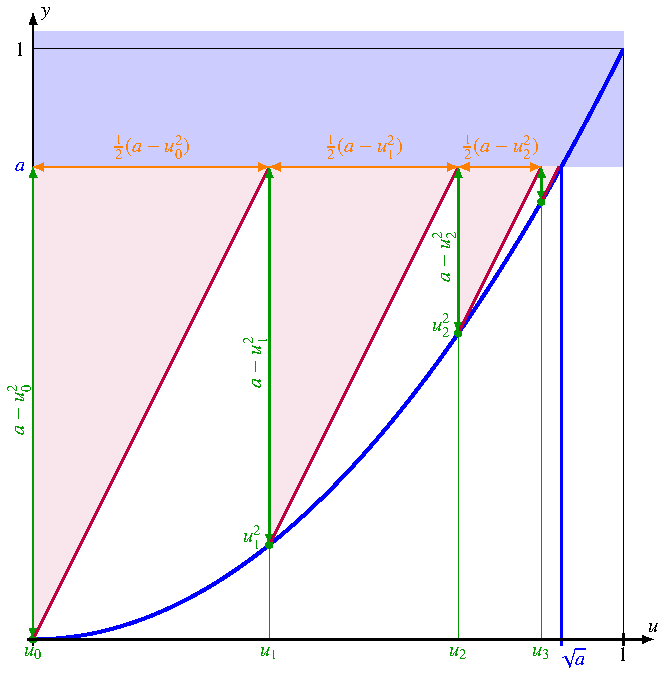
\includegraphics{chapters/40-eigenwerte/images/wurzel.pdf}
\caption{Konstruktion einer monoton wachsenden Approximationsfolge für
$\sqrt{a}$
\label{buch:eigenwerte:fig:wurzelverfahren}}
\end{figure}

\begin{figure}
\centering
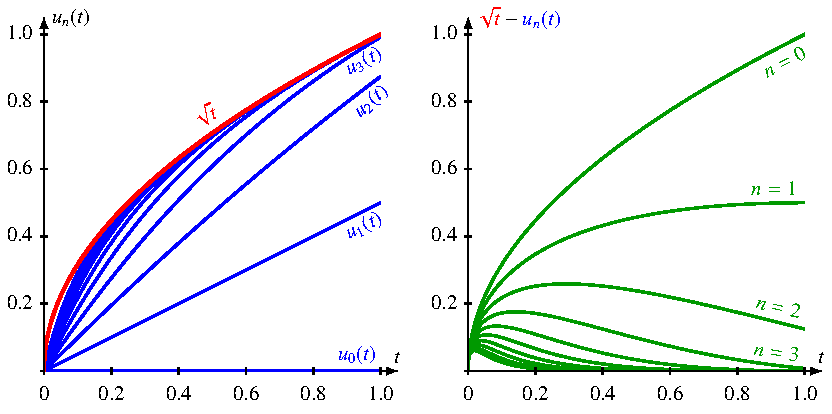
\includegraphics[width=\textwidth]{chapters/40-eigenwerte/images/wurzelapprox.pdf}
\caption{Monoton wachsende Approximation der Funktion $t\mapsto\sqrt{t}$ mit 
Polynomen $u_n(t)$ nach 
\eqref{buch:eigenwerte:eqn:wurzelapproximation}
(links) und der Fehler der Approximation
(rechts).
\label{buch:eigenwerte:fig:wurzelapproximation}}
\end{figure}

\begin{satz}[Stone-Weierstrass]
\label{buch:satz:stone-weierstrass}
Enthält eine $\mathbb{R}$-Algebra $A$ von stetigen, rellen Funktionen
auf einer kompakten Menge $K$ die konstanten Funktionen und trennt sie
Punkte, d.~h.~für zwei verschiedene Punkte $x,y\in K$ gibt es
immer eine Funktion $f\in A$ mit $f(x)\ne f(y)$, dann ist jede stetige,
reelle Funktion auf $K$ gleichmässig approximierbar durch Funktionen 
in $A$.
\end{satz}

Für den Beweis des Satzes wird ein Hilfsresultat benötigt, welches wir
zunächst ableiten.
Es besagt, dass sich die Wurzelfunktion $t\mapsto\sqrt{t}$
auf dem Interval $[0,1]$ gleichmässig
von unten durch Polynome approximieren lässt, die in
Abbildung~\ref{buch:eigenwerte:fig:wurzelapproximation} dargestellt
sind.

\begin{satz}
Die rekursiv definierte Folge von Polynomen
\begin{equation}
u_{n+1}(t)
=
u_n(t) + \frac12(t-u_n(t)^2),
\qquad
u_0(t)=0
\label{buch:eigenwerte:eqn:wurzelapproximation}
\end{equation}
ist monoton wachsend und approximiert die Wurzelfunktion $t\mapsto\sqrt{t}$
gleichmässig auf dem Intervall $[0,1]$.
\end{satz}

\begin{figure}
\centering
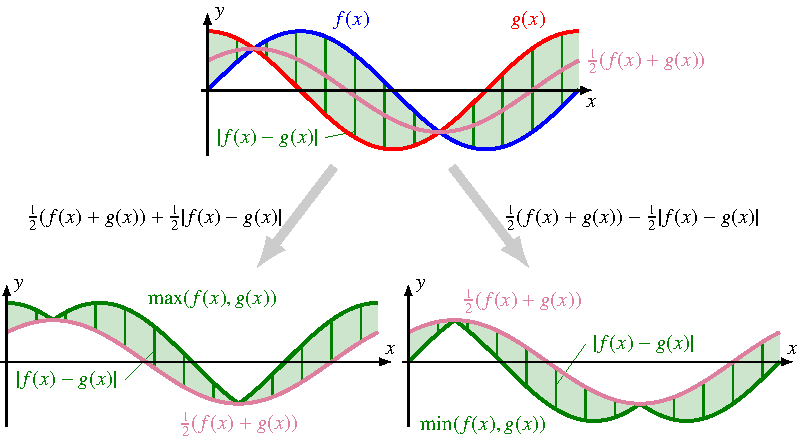
\includegraphics{chapters/40-eigenwerte/images/minmax.pdf}
\caption{Graphische Erklärung der
Identitäten~\eqref{buch:eigenwerte:eqn:minmax} für
$\max(f(x),g(x))$ und $\min(f(x),g(x))$.
Die purpurrote Kurve stellt den Mittelwert von $f(x)$ und $g(x)$ dar,
die vertikalen grünen Linien haben die Länge der Differenz $|f(x)-g(x)|$.
Das Maximum erhält man, indem man den halben Betrag der Differenz zum
Mittelwert hinzuaddiert, das Minimum erhält man durch Subtraktion
der selben Grösse.
\label{buch:eigenwerte:fig:minmax}}
\end{figure}

\begin{proof}[Beweis]
Wer konstruieren zunächst das in
Abbildung~\ref{buch:eigenwerte:fig:wurzelverfahren}
visualierte Verfahren, mit dem für jede Zahl $a\in[0,1]$
die Wurzel $\sqrt{a}$ berechnet werden kann.
Sei $u < \sqrt{a}$ eine Approximation der Wurzel.
Die Approximation ist der exakte Wert der Lösung, wenn $a-u^2=0$.
In jedem anderen Fall muss $u$ um einen Betrag $d$ vergrössert werden.
Natürlich muss immer noch $u+d<\sqrt{a}$ sein.
Man kann die maximal zulässige Korrektur $d$ geometrisch abschätzen,
wie dies in Abbildung~\ref{buch:eigenwerte:fig:wurzelverfahren}
skizziert ist.
Die maximale Steigung des Graphen der Funktion $u\mapsto u^2$ ist $2$,
daher darf man $u$ maximal um die Hälfte der Differenz $a-u^2$ (grün)
vergrössern, also $d=\frac12(a-u^2)$.
Die Rekursionsformel
\[
u_{n+1} = u_n + d = u_n + \frac12(a-u_n^2)
\]
mit dem Startwert $u_0=0$ liefert daher eine 
Folge, die gegen $\sqrt{a}$ konvergiert.
\end{proof}

\begin{proof}[Beweis des Satzes von Stone-Weierstrass]
Da $A$ eine Algebra ist, ist mit jeder Funktion $f\in A$ für jedes Polynome
$p\in\mathbb{R}[X]$ auch $p(f)$ eine Funktion in $A$.
\begin{enumerate}
\item Schritt: Für jede Funktion $f\in A$ lässt sich auch $|f|$ durch
Funktionen in $A$ beliebig genau durch eine monoton wachsende Folge
von Funktionen approximieren.

Da $A$ eine Algebra ist, ist $f^2\in A$.
Sei ausserdem $m^2=\sup \{f(x)^2\;|\;x\in K\}$, so dass $f^2/m^2$ eine Funktion
mit Werten im Intervall $[0,1]$ ist.
Die Funktionen $f_n(x)=mu_n(f(x)^2/m^2)$ sind ebenfalls in $A$ und
approximieren gleichmässig $\sqrt{f(x)^2}=|f(x)|$.
\item Schritt: Für zwei Funktionen $f,g\in A$ gibt es eine monoton wachsende
Folge, die $\max(f,g)$ gleichmässig beliebig genau approximiert
und eine monoton fallende Folge, die $\min(f,g)$ gleichmässig beliebig 
genau approximiert.


Diese Folgen können aus der Approximationsfolge für den Betrag einer
Funktion und den Identitäten
\begin{equation}
\begin{aligned}
\max(f,g) &= \frac12(f+g+|f-g|) \\
\min(f,g) &= \frac12(f+g-|f-g|) 
\end{aligned}
\label{buch:eigenwerte:eqn:minmax}
\end{equation}
gefunden werden, die in Abbildung~\ref{buch:eigenwerte:fig:minmax}
graphisch erklärt werden.
\item Schritt: Zu zwei beliebigen Punkten $x,y\in K$ und Werten
$\alpha,\beta\in\mathbb{R}$ gibt es immer eine Funktion in $A$,
die in den Punkten $x,y$ die vorgegebenen Werte $\alpha$ bzw.~$\beta$
annimmt.
Da $A$ die Punkte trennt, gibt es eine Funktion $f_0$ mit $f_0(x)\ne f_0(y)$.
Dann ist die Funktion
\[
f(t)
=
\beta + \frac{f_0(t)-f_0(y)}{f_0(x)-f_0(y)}(\alpha-\beta)
\]
wohldefiniert und nimmt die verlangten Werte an.
\item Schritt: Zu jeder stetigen Funktion $f\colon K\to\mathbb{R}$, jedem
Punkt $x\in K$ und jedem $\varepsilon>0$ gibt es eine Funktion $g\in A$ derart,
dass $g(x)=f(x)$ und $g(y) \le f(y)+\varepsilon$ für alle $y\in K$.

Zu jedem $z\in K$ gibt es eine Funktion in $A$ mit
$h_z(x)=f(x)$ und $h_z(z) \le f(z)+\frac12\varepsilon$.
Wegen der Stetigkeit von $h_z$ gibt es eine Umgebung $V_z$ von $z$, in der
immer noch gilt $h_z(y)\le f(y)+\varepsilon$ für $y\in V_z$.
Wegen der Kompaktheit von $K$ kann man endlich viele Punkte $z_i$ wählen
derart, dass die $V_{z_i}$ immer noch $K$ überdecken.
Dann erfüllt die Funktion
\(
g(z) = \inf h_{z_i}
\)
die Bedingungen $g(x) = f(x)$ und für $z\in V_{z_i}$
\[
g(z) = \inf_{j} h_{z_j}(z) \le h_{z_i}(z) \le f(z)+\varepsilon.
\]
Ausserdem ist $g(z)$ nach dem zweiten Schritt beliebig genau durch
Funktionen in $A$ approximierbar.
\item Schritt: Jede stetige Funktion $f\colon K\to\mathbb{R}$ kann
beliebig genau durch Funktionen in $A$ approximiert werden.
Sei $\varepsilon > 0$.

Nach dem vierten Schritt gibt es für jedes $y\in K$ eine Funktion $g_y$
derart, dass $g_y(y)=f(y)$  und $g_y(x) \le f(x) + \varepsilon$ für
$x\in K$.
Da $g_y$ stetig ist, gilt ausserdem $g_y(x) \ge f(x) -\varepsilon$ in
einer Umgebung $U_y$ von $y$.
Da $K$ kompakt ist, kann man endlich viele $y_i$ derart, dass die $U_{y_i}$
immer noch ganz $K$ überdecken.
Die Funktion $g=\sup g_{y_i}$ erfüllt dann überall $g(x) \le f(x)+\varepsilon$,
weil jede der Funktionen $g_y$ diese Ungleichung erfüllt.
Ausserdem gilt für $x\in V_{x_j}$
\[
g(x) = \sup_i g_{x_i}(x) \ge g_{x_j}(x) \ge f(x)-\varepsilon.
\]
Somit ist
\[
|f(x)-g(x)| \le \varepsilon.
\]
Damit ist $f(x)$ beliebig nahe an der Funktion $g(x)$, die sich 
beliebig genau durch Funktionen aus $A$ approximieren lässt.
\qedhere
\end{enumerate}
\end{proof}

Im ersten Schritt des Beweises ist ganz entscheidend, dass man die
Betragsfunktion konstruieren kann.
Daraus leiten sich dann alle folgenden Konstruktionen ab.

\subsubsection{Anwendung auf symmetrische und hermitesche Matrizen}
Für symmetrische und hermitesche Matrizen $A$ ist bekannt, dass die
Eigenwerte reell sind, also das Spektrum $\operatorname{A}\subset\mathbb{R}$
ist.
Für eine Funktion $\mathbb{R}\to \mathbb{R}$ lässt sich nach dem
Satz~\ref{buch:satz:stone-weierstrass} immer eine Folge $p_n$ von
approximierenden Polynomen in $x$ finden, die auf $\operatorname{Sp}(A)$
gleichmässig konvergiert.
Die Matrix $f(A)$ kann dann definiert werden also der Grenzwert
\[
f(A) = \lim_{n\to\infty} p_n(A).
\]
Da diese Matrizen auch diagonalisierbar sind, kann man eine Basis
aus Eigenvektoren verwenden.
Die Wirkung von $p_n(A)$ auf einem Eigenvektor $v$ zum Eigenwert $\lambda$
ist
\[
p_n(A)v
=
(a_kA^k + a_{k-1}A^{k-1}+\dots +a_2A^2+a_1A+a_0I)v
=
(a_k\lambda^k + a_{k-1}\lambda^{k-1}+\dots + a_2\lambda^2 + a_1\lambda + a_0)v
=
p_n(\lambda)v.
\]
Im Grenzwert wirkt $f(A)$ daher durch Multiplikation eines Eigenvektors
mit $f(\lambda)$, die Matrix $f(A)$ hat in der genannten Basis die
Diagonalform
\[
A=\begin{pmatrix}
\lambda_1&         &      &         \\
         &\lambda_2&      &         \\
         &         &\ddots&         \\
         &         &      &\lambda_n
\end{pmatrix}
\qquad\Rightarrow\qquad
f(A)=\begin{pmatrix}
f(\lambda_1)&            &      &            \\
            &f(\lambda_2)&      &            \\
            &            &\ddots&            \\
            &            &      &f(\lambda_n)
\end{pmatrix}.
\]

\begin{satz}
\label{buch:eigenwerte:satz:spektralsatz}
Ist $A$ symmetrische oder selbstadjungiert Matrix und $f$ eine Funktion
auf dem Spektrum $\operatorname{Sp}(A)$ von $A$.
Dann gibt es genau eine Matrix $f(A)$, die Grenzwert jeder beliebigen
Folge $p_n(A)$ für Polynomfolgen, die $\operatorname{Sp}(A)$ gleichmässig
gegen $f$ konvergieren.
\end{satz}

\subsubsection{Unmöglichkeit der Approximation von $z\mapsto \overline{z}$
in $\mathbb{C}[z]$}
Der Satz~\ref{buch:satz:stone-weierstrass} von Stone-Weierstrass für
reelle Funktionen gilt nicht für komplexe Funktionen.
In diesem Abschnitt zeigen wir, dass sich die Funktion $z\mapsto\overline{z}$
auf der Einheitskreisscheibe $K=\{z\in\mathbb{C}\;|\; |z|\le 1\}$ nicht
gleichmässig durch Polynome $p(z)$ mit komplexen Koeffizienten approximieren
lässt.

Wäre eine solche Approximation möglich, dann könnte man $\overline{z}$
auch durch eine Potenzreihe
\[
\overline{z}
=
\sum_{k=0}^\infty a_kz^k
\]
darstellen.
Das Wegintegral beider Seiten über den Pfad $\gamma(t) = e^{it}$
in der komplexen Ebene ist
\begin{align*}
\oint_\gamma z^k\,dz
&=
\int_0^{2\pi} e^{ikt} ie^{it}\,dt
=
i\int_0^{2\pi} e^{it(k+1)}\,dt
=
i\biggl[ \frac{1}{i(k+1)} e^{it(k+1)}\biggr]_0^{2\pi}
=
0
\\
\oint_\gamma
\sum_{k=0}^\infty a_kz^k
\,dz
&=
\sum_{k=0}^\infty a_k \oint_\gamma z^k\,dz
=
\sum_{k=0}^\infty a_k\cdot 0
=
0
\\
\oint_\gamma \overline{z}\,dz
&=
\int_0^{2\pi} e^{it} ie^{it}\,dt
=
i\int_0^{2\pi} \,dt = 2\pi i,
\end{align*}
dabei wurde $\overline{\gamma}(t)=e^{-it}$ verwendet.
Insbesondere widersprechen sich die beiden Integrale.
Die ursprüngliche Annahmen, $\overline{z}$ lasse sich durch Polynome
gleichmässig approximieren, muss daher verworfen werden.

\subsubsection{Der Satz von Stone-Weierstrass für komplexe Funktionen}
Der Satz von Stone-Weierstrass kann nach dem vorangegangene Abschnitt
also nicht gelten.
Um den Beweis des Satzes~\ref{buch:satz:stone-weierstrass}
auf komplexe Zahlen zu übertragen, muss im ersten Schritt ein Weg
gefunden werden, den Betrag einer Funktion zu approximieren.

Im reellen Fall geschah dies, indem zunächst eine Polynom-Approximation
für die Quadratwurzel konstruiert wurde, die dann auf das Quadrat einer
Funktion angewendet wurde.
Der Betrag einer komplexen Zahl $z$ ist aber nicht allein aus $z$
berechenbar, man braucht in irgend einer Form Zugang zu Real-
und Imaginärteil.
Zum Beispiel kann man Real- und Imaginärteil als
$\Re z= \frac12(z+\overline{z})$ und $\Im z = \frac12(z-\overline{z})$
bestimmen.
Kenntnis von Real- und Imaginärteil ist als gleichbedeutend mit
der Kenntnis der komplex Konjugierten $\overline{z}$.
Der Betrag lässt sich daraus als $|z|^2 = z\overline{z}$ finden.
Beide Beispiele zeigen, dass man den im Beweis benötigten Betrag
nur dann bestimmen kann, wenn mit jeder Funktion aus $A$ auch die
komplex konjugierte Funktion zur Verfügung steht.

\begin{satz}[Stone-Weierstrass]
Enthält eine $\mathbb{C}$-Algebra $A$ von stetigen, komplexwertigen
Funktionen auf einer kompakten Menge $K$ die konstanten Funktionen,
trennt sie Punkte und ist ausserdem mit jeder Funktion $f\in A$ auch
die komplex konjugiert Funktion $\overline{f}\in A$,
dann lässt sich jede stetige, komplexwertige Funktion 
auf $K$ gleichmässig durch Funktionen aus $A$ approximieren.
\end{satz}

Mit Hilfe der konjugiert komplexen Funktion lässt sich immer eine
Approximation für die Betragsfunktion finden, so dass sich der
Beweis des reellen Satzes von Stone-Weierstrass übertragen lässt.

%
% Normale Matrizen
%
\subsection{Normale Matrizen
\label{buch:subsection:normale-matrizen}}
Aus dem Satz von Stone-Weierstrass für komplexe Matrizen kann man
jetzt einen Spektralsätze für eine etwas grössere Klasse von Matrizen
ableiten, als im Satz~\ref{buch:eigenwerte:satz:spektralsatz}
möglich war.
Der Satz besagt, dass für eine beliebige Funktion $f$ auf dem Spektrum
$\operatorname{Sp}(A)$ eine Folge von auf $\operatorname{Sp}(A)$
gleichmässig konvergenten, approximierenden Polynomen
$p_n(z,\overline{z})$ gefunden werden kann.
Doch wie soll jetzt aus dieser Polynomfolge ein Kandidat von $f(A)$
gefunden werden?

Zunächst stellt sich die Frage, was für die Variable $\overline{z}$ 
eingesetzt werden soll.
$1\times 1$-Matrizen sind notwendigerweise diagonal, also muss 
man in diesem Fall die Matrix $\overline{A}$ für die Variable
$\overline{z}$ eingesetzt werden.
Dies erklärt aber noch nicht, wie für $n\times n$-Matrizen
vorzugehen ist, wenn $n>1$ ist.

Die Notwendigkeit, die Variable $\overline{z}$ hinzuzunehmen
ergab sich aus der Anforderung, dass der Betrag aus $|z|^2=z\overline{z}$
konstruiert werden können muss.
Insbesondere muss beim Einsetzen eine Matrix entstehen, die nur 
positive Eigenwerte hat.
Für eine beliebige komplexe $n\times n$-Matrix $A$ ist aber
$A\overline{A}$ nicht notwendigerweise positiv, wie das Beispiel
\[
A
=
\begin{pmatrix}0&i\\i&0\end{pmatrix}
\qquad
\Rightarrow
\qquad
A\overline{A}
=
\begin{pmatrix}0&i\\-i&0\end{pmatrix}
\begin{pmatrix}0&-i\\i&0\end{pmatrix}
=
\begin{pmatrix}
-1&0\\
 0&-1
\end{pmatrix}
=
-I
\]
zeigt.
Eine positive Matrix entsteht dagegen immer, wenn man statt
$A$ die Adjungierte $A^*=\overline{A}^t$ verwendet.

Die Substitution von $A$ für $z$ und $A^*$ für $\overline{z}$
in einem Polynom $p(z,\overline{z})$ ist nicht unbedingt eindeutig.
Schon das Polynom $p(z,\overline{z})=z\overline{z}$ kann man auch
als $\overline{z}z$ schreiben.
Damit die Substition eindeutig wird, muss man also fordern, dass
$AA^* = A^*A$ ist.

\begin{definition}
Eine Matrix $A\in M_n(\mathbb{C})$ heisst {\em normal}, wenn $AA^*=A^*A$ gilt.
\end{definition}

\subsubsection{Beispiele normaler Matrizen}

\begin{enumerate}
\item
Hermitesche und Antihermitesche Matrizen sind normal, denn solche
Matrizen erfüllen $A^*=\pm A$ und damit
\(
AA^* = \pm A^2 = A^*A.
\)
\item
Symmetrische und antisymmetrische Matrizen sind normal,
denn aus $A=A^t$ folgt $A^*=\overline{A}^t$ und damit
\begin{align*}
AA^* &=  A\overline{A}^t = 
\\
A^*A &=
\end{align*}
\item
Unitäre Matrizen $U$ sind normal, das $UU^*=I=U^*U$ gilt.
\item
Orthogonale Matrizen sind normal wegen $O(n) = U(n) \cap M_n(\mathbb{R})$.
\end{enumerate}

Jede Matrix lässt sich durch Wahl einer geeigneten Basis in Jordansche 
Normalform bringen.
Allerdings sind Jordan-Blöcke keine normalen Matrizen, wie der folgende
Satz zeigt.

\begin{satz}
Eine Dreiecksmatrix ist genau dann normal, wenn sie diagonal ist.
\end{satz}

\begin{proof}[Beweis]
Sei $A$ eine obere Dreiecksmatrix, das Argument für eine untere Dreiecksmatrix
funktioniert gleich.
Wir berechnen ein Diagonalelement für beide Produkte $AA^*$ und $A^*A$.
Dazu brauchen wir die Matrixelemente von $A$ und $A^*$.
Bezeichnen wir die Matrixelemente von $A$ mit $a_{ij}$, dann hat $A^*$
die Matrixelemente $(A^*)_{ij}=\overline{a}_{ji}$.
Damit kann man die Diagonalelemente der Produkte als
\begin{align*}
(AA^*)_{ii}
&=
\sum_{j=1}^n a_{ij}\overline{a}_{ij}
=
\sum_{j=i}^n |a_{ij}|^2
\\
(A^*A)_{ii}
&=
\sum_{j=1}^n \overline{a}_{ji}a_{ji}
=
\sum_{j=1}^i |a_{ji}|^2
\end{align*}
ausrechnen.
Der obere Ausdruck ist die quadrierte Länge der Zeile $i$ der Matrix $A$,
der untere ist die quadrierte Länge der Spalte $i$.
Da die Matrix eine obere Dreiecksmatrix ist, hat die erste Spalte höchstens
ein einziges von $0$ verschiedenes Element.
Daher kann auch die erste Zeile höchstens dieses eine Elemente haben.
Die Matrix hat daher Blockstruktur mit einem $1\times 1$-Block in der
linken obere Ecke und einem  $n-1$-dimensionalen Block für den Rest.
Durch Wiederholen des Arguments für den $(n-1)\times (n-1)$-Block 
kann man so schrittweise schliessen, dass die Matrix $A$ diagonal sein muss.
\end{proof}


\begin{satz}
Sind $A$ und $B$ normale Matrizen und $AB^*=B^*A$, dann sind auch $A+B$
und $AB$ normal.
\end{satz}

\begin{proof}[Beweis]
Zunächst folgt aus $AB^*=B^*A$ auch
$A^*B = (B^*A)^* = (AB^*)^* = BA^*$.
Der Beweis erfolgt durch Nachrechnen:
\begin{align*}
(A+B)(A+B)^*
&=
AA^* + AB^* + BA^*+BB^*
\\
(A+B)^*(A+B)
&=
A^*A + A^*B + B^*A + B^*B
\end{align*}
Die ersten und letzten Terme auf der rechten Seite stimmen überein, weil
$A$ und $B$ normal sind.
Die gemischten Terme stimmen überein wegen der Vertauschbarkeit von
$A$ und $B^*$.

Für das Produkt rechnet man
\begin{align*}
(AB)(AB)^*
&= ABB^*A^* = AB^*BA^*
= B^*AA^*B
=
B^*A^*AB
=
(AB)^*(AB),
\end{align*}
was zeigt, dass auch $AB$ normal ist.
\end{proof}

\subsubsection{Äquivalente Bedingungen}
Es gibt eine grosse Zahl äquivalenter Eigenschaften für normale Matrizen.
Die folgenden Eigenschaften sind äquivalent:
\begin{enumerate}
\item
Die Matrix $A$ ist mit einer unitären Matrix diagonalisierbar
\item
Es gibt eine orthonormale Basis von Eigenvektoren von $A$ für $\mathbb{C}^n$
\item
Für jeden Vektor $x\in\mathbb{C}^n$ gilt $\|Ax\|=\|A^*x\|$
\item
Die Forbenius-Norm der Matrix $A$ kann mit den Eigenwerten $\lambda_i$
von $A$ berechnet werden:
$\operatorname{Spur}(A^*A) = \sum_{i=1}^n |\lambda_i|^2$
\item
Der hermitesche Teil $\frac12(A+A^*)$ und der antihermitesche Teil
$\frac12(A-A^*)$ von $A$ vertauschen.
\item
$A^*$ ist ein Polynom vom Grad $n-1$ in $A$.
\item
Es gibt eine unitäre Matrix $U$ derart, dass $A^*=AU$
\item
Es gibt eine Polarzerlegugn $A=UP$ mit einer unitären Matrix $U$ und
einer postiv semidefiniten Matrix $P$, die untereinander vertauschen.
\item
Es gibt eine Matrix $N$ mit verschiedenen Eigenwerten, mit denen $A$
vertauscht.
\item
Wenn $A$ die (absteigend geordneten) singulärwerte $\sigma_i$ und
die absteigend geordneten Eigenwerte $\lambda_i$ hat,
dann it $\sigma_i=|\lambda_i|$.
\end{enumerate}





%%
% numerisch.tex
%
% (c) 2020 Prof Dr Andreas Müller, Hochschule Rapeprswil
%
\section{Numerische Verfahren zur Eigenwertbestimmung
\label{buch:section:numerische-verfahren-eigenwerte}}
% Jacobi-Algorithmus
% Potenzverfahren
% Francis-Algorithmus



\section*{Übungsaufgaben}
\rhead{Übungsaufgaben}
\aufgabetoplevel{chapters/40-eigenwerte/uebungsaufgaben}
\begin{uebungsaufgaben}
\uebungsaufgabe{4001}
\uebungsaufgabe{4002}
\uebungsaufgabe{4003}
\uebungsaufgabe{4004}
\uebungsaufgabe{4005}
\uebungsaufgabe{4006}
\end{uebungsaufgaben}

